%=========================================================================
% (c) Michal Bidlo, Bohuslav Křena, 2008
% Text napsala Dominika Regeciova

%%%%%%%%%%%%%%%%%%%%%%%%%%%%%%%%%%%%%%%%%%%%%%%%%%%%%%%%%%%%%%%%%%%%%%%%%%%%%%%%%%%%%%%%%%%%%%%%%%%%%%%%%%%%%%%%%%%%%%%%%%%%%%%%%%%%%%%%%%%%%%%%%%%%%
% 1. Kapitola
%%%%%%%%%%%%%%%%%%%%%%%%%%%%%%%%%%%%%%%%%%%%%%%%%%%%%%%%%%%%%%%%%%%%%%%%%%%%%%%%%%%%%%%%%%%%%%%%%%%%%%%%%%%%%%%%%%%%%%%%%%%%%%%%%%%%%%%%%%%%%%%%%%%%%
\chapter{Úvod}\label{ch:introduction}
Studium počítačové bezpečnosti může být poněkud deprimující záležitostí. Každým okamžikem nás zaplavují nové informace o~zranitelných místech, 
chybách v~aplikacích a případech útoků, které byly provedeny často na nebezpečně kritických systémech, kdy cílem mohou být například jaderné 
elektrárny, elektrické rozvodné sítě\footnote{\url{www.wired.com/story/hack-brief-us-nuclear-power-breach/}}, nebo i 
nemocnice\footnote{\url{www.bleepingcomputer.com/news/security/bit-paymer-ransomware-hits-scottish-hospitals/}}.\\

Jedno z~mnoha závažných ohrožení bezpečnosti bylo uveřejněno v~srpnu roku 2017, kdy \mbox{\textit{U.S. Food and Drug Administration}} (FDA) vyzvala 
skoro půl miliónu pacientů s~kardiostimulátory k~aktualizaci firmwaru. Byla v~něm totiž nalezena zranitelnost, která umožňovala neautorizované úpravy 
nastavení, které by mohly vést k~ohrožení zdraví pacientů\footnote{\url{www.fda.gov/MedicalDevices/Safety/AlertsandNotices/ucm573669.htm}}. \\

Je jednoduché dostat se do stavu, kdy se cítíme doslova obklopeni hrozbami a snad jedinou bezpečnou ochranou je přetrvat po zbytek života 
v~kamenné jeskyni. V~amazonském pralese. S~dostatečným množstvím alobalu. Protože si nemůžeme být nikdy dostatečně jisti. \\

Mnoho vysoce kvalifikovaných lidí na celém světě neustále pracují na tom, aby náš přetechnizovaný svět udělali bezpečnějším místem, ale jako by vedli 
nekonečný závod se záškodníky, kteří mají bohužel většinou náskok. Opravdu je to nekončící boj? Opravdu jsme uvězněni v~nekonečném kolotoči objevování 
nových a nových zranitelností a chyb, jejich náročných oprav, abychom poté začali zase od znova? \\

Myslím, že nejsem jediná, kdo vnímá celou situaci kolem bezpečnosti jako ve stavu odevzdané defenzivy. Jako by se experti smířili s~tím, že bezpečný 
systém je něco jako \textit{jednorožec} ve světě techniky --- krásná, ale nerealistická záležitost. Proto není otázkou, zda se najdou chyby, ale kdy 
se projeví a kdo je objeví první --- zda ti dobří, nebo zlí. Následně se chyba opraví, pokud možno dobře a zase nastává doba ticha před bouří. \\

I~proto jsem byla překvapena, když jsem objevila článek \textit{Security Applications of Formal Language Theory} \cite{Sass2013}. Zde je totiž zmíněna 
pro mě v~té době nová myšlenka: zranitelnosti a chyby v~systému jsou jako moc, kterou dáváme na pospas světu. A~dáváme ji dobrovolně. Například v~podobě 
výpočetní síly. Špatně zvolené gramatiky. Nebo prostě jen myšlenky, že bychom měli být liberální k~tomu, co přijímáme z~okolí \cite[str. 1]{Geer2010}. \\

V~této práci se předpokládá čtenářova základní znalost z~oboru teoretické informatiky, především z~oblasti teorie formálních jazyků. V~\ref{ch:theory}. 
kapitole i přesto pro připomenutí budou zmíněny základní a klíčové pojmy pro tuto práci, především Chomského hierarchie a síla jednotlivých jazyků dle 
tohoto členění. Protože je téma tak svázané se světem bezpečnosti, bude věnována i ji úvodní část, přesněji \ref{ch:security}. kapitola, pro krátké 
stanovení častých pojmů, které budou v~práci používány. Pokud bude zmíněn konkrétní případ zranitelnosti, či vybraný útok, bude vždy následovat krátké 
obeznámení s~danou problematikou, popřípadě odkaz na doplňující literaturu, pokud by čtenář toužil vědět více. \\

Po dvou úvodních kapitolách si představíme přístup, který se stal základem pro tuto diplomovou práci. Uvedeme si, v~čem spočívá výjimečnost 
\textit{LangSecu} (kapitola \ref{ch:langsec}) a jeho bezpečnostních zásad včetně jeho vývoje od roku 2011. To, že se nejedná pouze o~teoretický koncept, 
si ukážeme na příkladech reálného použití v~kapitole \ref{ch:langsecapp}. V~\ref{ch:sqlifirewall}. kapitole si pak představíme aplikaci, která bude 
rovněž používat tohoto přístupu. Uvedeme si postup implementace a otestujeme přínosy oproti klasickým metodám vývoje. 
Na závěr, v~kapitole~\ref{ch:vysledky}, si shrneme dosažené výsledky a vyhodnotíme, jaký může mít prospěch využívat teorie formálních jazyků při 
zajišťování počítačové bezpečnosti. \\

Protože je práce psaná v~českém jazyce, jsou termíny uváděny podle zažité české terminologie, kdy při prvním použití bude anglický ekvivalent uveden 
v~závorkách. Jako hlavním zdrojem pro kontrolu byla využita publikace \textit{Výkladový slovník kybernetické bezpečnosti}~\cite{Slovnik2015}. 
Existuje však řada pojmů, která zavedený český ekvivalent nemá, nebo je ho v~praxi používáno minimálně, proto budeme tyto pojmy uvádět v~originální 
podobě (například \textit{software}, \textit{exploit}, nebo již zmiňovaný \textit{firmware}). Slovník nejčastějších termínů včetně krátkého
vysvětlení lze nalézt v~příloze \ref{app:concepts}. \\

Teorii formálních jazyků, ale nejen tu, bude provázet řada příkladů. Pro jejich označení bude vždy sloužit symbol \Bat.

%%%%%%%%%%%%%%%%%%%%%%%%%%%%%%%%%%%%%%%%%%%%%%%%%%%%%%%%%%%%%%%%%%%%%%%%%%%%%%%%%%%%%%%%%%%%%%%%%%%%%%%%%%%%%%%%%%%%%%%%%%%%%%%%%%%%%%%%%%%%%%%%%%%%%
% 2. Kapitola
%%%%%%%%%%%%%%%%%%%%%%%%%%%%%%%%%%%%%%%%%%%%%%%%%%%%%%%%%%%%%%%%%%%%%%%%%%%%%%%%%%%%%%%%%%%%%%%%%%%%%%%%%%%%%%%%%%%%%%%%%%%%%%%%%%%%%%%%%%%%%%%%%%%%%
\chapter{Teoretický úvod} \label{ch:theory}
Teorie formálních jazyků představuje podstatnou součást teoretické informatiky. Pro~další kapitoly je porozumění této oblasti klíčové, především pak 
určování algoritmické řešitelnosti --- tedy zda můžeme dosáhnout výsledků v~konečném čase. Než si ale vysvětlíme, jak zasahuje teorie formálních 
jazyků do problematiky bezpečnosti, projdeme si nejdůležitější poznatky, kterých následně budeme hojně využívat. \\

Ať už pracujeme s~přirozenými jazyky, jakými jsou například čeština a angličtina, nebo s~jinými, například programovacími, chápeme související pojem 
gramatika intuitivně jako souhrn pravidel, podle kterých tyto jazyky vytváříme. Pro jejich zápis používáme \textit{terminální symboly}, které jsou 
tvořeny abecedou popisovaného jazyka a \textit{neterminální symboly}, pomocné proměnné, které většinou značíme pomocí velkých písmen. \\

\textbf{Gramatika} $G$ je čtveřice $G = (N, \Sigma, P, S)$, kde
\begin{itemize}
\item $N$ je konečná množina neterminálních symbolů
\item $\Sigma$ je konečná množina terminálních symbolů, $N \cap \Sigma = \emptyset$
\item $P$ je konečná podmnožina kartézského součinu $(N\cup\Sigma)^*N(N\cup\Sigma)^*\times(N\cup\Sigma)^*$
\item $S \in N$ je výchozí (také počáteční) symbol gramatiky
\end{itemize}
\vspace*{\baselineskip}
Prvek $(\alpha, \beta)$ množiny $P$ nazýváme \textit{přepisovacím pravidlem} (krátce \textit{pravidlem}) a budeme jej zapisovat 
ve tvaru $\alpha \rightarrow \beta$. Řetězec $\alpha$ resp. $\beta$ nazývám \textit{levou} resp. \textit{pravou stranou} přepisovacího 
pravidla \cite[str. 13]{TIN2013}. \\

Řetězce generované z~počátečního symbolu a obsahující terminální i neterminální symboly nazýváme \textit{větnými formami} \cite[str. 15]{TIN2013}. \\

\textbf{Jazyk} pak definujeme jako množinu všech řetězců generovaných gramatikou z~počátečního symbolu a obsahující pouze terminální symboly 
(tzv. \textit{věty}) \cite[str. 15]{TIN2013}. \\

Protože jsou jazyky množinami, lze nad nimi provádět operace definované nad množinami.
Můžeme určit sjednocení jazyků, jejich průnik, definovat komplement jazyka i jeho iteraci. Další operace nad jazyky jsou definovány následovně: \\

\textbf{Konkatenace} \\
Nechť $L_1$ je jazyk nad abecedou $\Sigma_1$, $L_2$ jazyk nad abecedou $\Sigma_2$. \textit{Součinem} (konkatenací) jazyků 
$L_1$ a $L_2$ je jazyk $L_1 \cdot L_2$ nad abecedou $\Sigma_1 \cup \Sigma_2$, jenž je definován takto:
\begin{center}
$L_1 \cdot L_2 = \{xy \ | \ x \in L_1, \ y \in L_2\}$
\end{center}
Operace součin jazyků je definována prostřednictvím konkatenace řetězců a má stejné vlastnosti jako konkatenace řetězců --- je asociativní 
a nekomutativní \cite[str. 10]{TIN2013}. \\

\textbf{Substituce jazyků} \\
Nechť $\pazocal{L}$ je třída jazyků a nechť $L \subseteq \Sigma^*$ je jazykem třídy $\pazocal{L}$. Dále nechť 
$\Sigma = \{a_1, a_2, \dots, a_n\}$ 
pro nějaké $n\in \mathbb{N}$ a nechť jazyky označené $L_{a_1}, L_{a_2}, \dots, L_{a_n}$ jsou rovněž jazyky třídy 
$\pazocal{L}$. Říkáme, že třída $\pazocal{L}$ je uzavřena vzhledem k~\textit{substituci}, jestliže pro každý výběr jazyků 
$L, L_{a_1}, L_{a_2}, \dots, L_{a_n}$ je také jazyk 
$\sigma_{L_{a_1}, L_{a_2}, \dots, L_{a_n}}(L)$
\begin{center}
$\sigma_{L_{a_1}, L_{a_2}, \dots, L_{a_n}}(L) = \{x_1 x_2 \dots x_m \ | \ b_1 b_2 \dots b_m \in L \wedge \forall i \in 
\{1, \dots, m\}: x_i \in L_{b_i}\}$ 
\end{center}
ve třídě $\pazocal{L}$ \cite[str. 95]{TIN2013}. \\

\textbf{Morfismus jazyků} \\
Nechť $\Sigma$ a $\Delta$ jsou abecedy a $L \subseteq \Sigma^*$ je jazyk nad abecedou $\Sigma$. Zobrazení $h: \Sigma^* \rightarrow \Delta^*$ 
nazveme morfismem nad slovy, platí-li $\forall w = a_1 a_2 \dots a_n \in \Sigma^*: h(w) = h(a_1) h(a_2) \dots h(a_n)$. 
\textit{Morfismus jazyka} $h(L)$ pak definujeme jako $h(L) = \{h(w) \ | \ w \in L\}$. \\ 
Morfismus jazyků je zvláštní případ substituce, kde každý substituovaný jazyk má právě jednu větu \cite[str. 95]{TIN2013}. \\

Při práci s~jazyky a jejich třídami nás zajímá řada otázek, přičemž především potřebujeme vědět, zda na danou otázku dokážeme odpovědět, a to 
v~konečném čase. Pokud je můžeme vyřešit pomocí konečného algoritmického řešení, označujeme je jako \textit{rozhodnutelné problémy}. 
V~opačném případě se jedná o~\textit{nerozhodnutelné problémy}. \\

Mezi tyto otázky se například řadí:
\begin{itemize}
\item Problém neprázdnosti, zda jazyk je, či není roven prázdné množině ($L \neq \emptyset$?)
\item Problém konečnosti jazyka $L(G)$
\item Problém náležitosti, tedy zda daný řetězec patří do jazyka, či nikoliv ($w \in L$?)
\item Problém ekvivalence, pokud máme dvě gramatiky $G_1$, $G_2$ a máme určit, zda generují stejný jazyk ($L(G_1) = L(G_2)$?)
\item Problém inkluze jazyků gramatik ($L(G_1) \subseteq L(G_2)$?)
\end{itemize}
\vspace*{\baselineskip}
Pro určení, pro jaké jazyky umíme vyřešit tyto problémy, nám pomáhá \textit{Chomského klasifikace gramatik}.

\section{Chomského klasifikace gramatik} \label{sec:2:chomsky}
\textbf{Avram Noam Chomsky} (* 1928) zavedl hierarchii gramatik a jazyků, ve které rozděluje gramatiky na 4 typy dle tvaru pravidel v~množině 
$P$ a které nám pomáhají určovat popisnou a rozhodovací sílu generovaných jazyků. \\

\textbf{Typ 0} \\
Gramatika typu 0 obsahuje pravidla v~nejobecnějším tvaru, shodným s~definicí gramatiky:
\begin{center}
$\alpha \rightarrow \beta, \ \alpha \in (N \cup \Sigma)^*N(N \cup \Sigma)^*, \ \beta \in (N \cup \Sigma)^*$
\end{center}
Z~tohoto důvodu se gramatiky typu 0 nazývají také gramatikami \textit{neomezenými} \cite[str. 16]{TIN2013}. \\
\newpage
\textbf{Typ 1} \\
Gramatika typu 1 obsahuje pravidla tvaru:
\begin{center}
$ \alpha A \beta \rightarrow \alpha\gamma\beta, \ A \in N, \ \alpha, \beta \in (N \cup \Sigma)^*, \ \gamma \in (N \cup \Sigma)^+$ 
\end{center}
nebo
\begin{center}
$ S \rightarrow \epsilon$ 
\end{center}
pokud se $S$ neobjevuje na pravé straně žádného pravidla. Gramatiky typu 1 se nazývají také gramatikami 
\textit{kontextovými} \cite[str. 16]{TIN2013}. \\

\textbf{Typ 2} \\
Gramatika typu 2 obsahuje pravidla tvaru:
\begin{center}
$ A \rightarrow \gamma, \ A \in N, \ \gamma \in (N \cup \Sigma)^*$
\end{center}
Gramatiky typu 2 se nazývají \textit{bezkontextovými} gramatikami \cite[str. 17]{TIN2013}. \\

\textbf{Typ 3} \\
Gramatika typu 3 obsahuje pravidla tvaru:
\begin{center}
$ A \rightarrow aB$ \ nebo \ $A \rightarrow a; \ A,B \in N, \ a \in \Sigma$
\end{center}
nebo
\begin{center}
$ S \rightarrow \epsilon$
\end{center}
pokus se $S$ neobjevuje na pravé straně žádného pravidla. Gramatika s~tímto tvarem pravidel se nazývá \textit{(pravá) regulární} 
gramatika \cite[str. 17]{TIN2013}. \\

Jazyky generované těmito gramatikami nazýváme následovně: \textit{rekurzivně vyčíslitelné} \mbox{(typ 0)}, \textit{kontextové}
(typ 1), \textit{bezkontextové} (typ 2) a \textit{regulární} (typ 3). Pro třídy těchto jazyků $\pazocal{L}_i, i = 0, 1, 2, 3$ 
platí $\pazocal{L}_3 \subset \pazocal{L}_2 \subset \pazocal{L}_1 \subset \pazocal{L}_0$ 
\cite[str. 18]{TIN2013}, jak je naznačeno na obrázku \ref{fig:chomsky}. \\

\begin{figure}[h!]
    \label{fig:chomsky}
    \centering
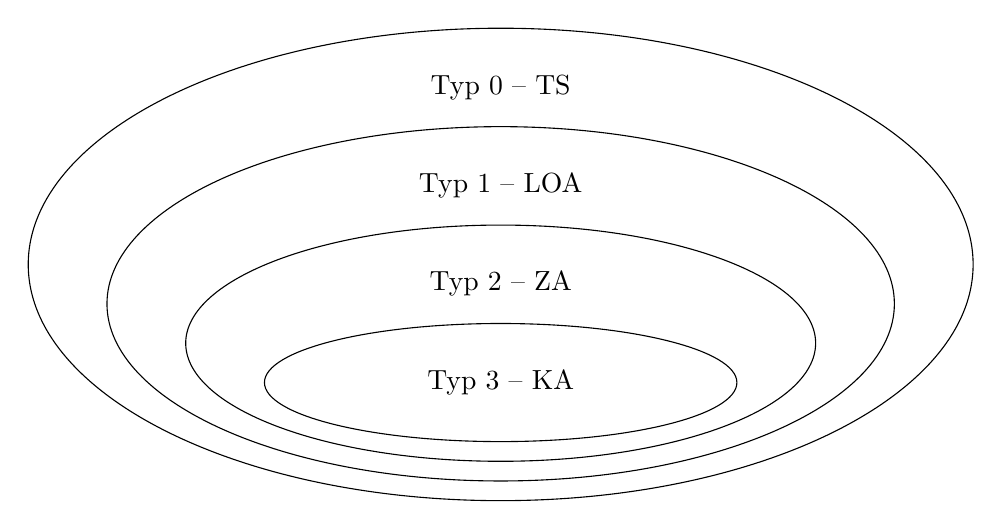
\begin{tikzpicture}
\draw [color=black] (7,5.5) ellipse [x radius = 6, y radius = 3];
\draw [color=black] (7,5) ellipse [x radius = 5, y radius = 2.25];
\draw [color=black] (7,4.5) ellipse [x radius = 4, y radius = 1.5];
\draw [color=black] (7,4) ellipse [x radius = 3, y radius = 0.75];
\node [at = {(7,7.75)}] {Typ 0 -- TS};
\node [at = {(7,6.5)}] {Typ 1 -- LOA};
\node [at = {(7,5.25)}] {Typ 2 -- ZA};
\node [at = {(7,4)}] {Typ 3 -- KA};
\end{tikzpicture}
    \caption{Graf Chomského hierarchie: třídy gramatik a automaty, které je přijímají}
\end{figure}
\newpage
\section{Regulární jazyky} \label{sec:2:reg}
Jazyk nad abecedou je regulární, pokud může být získán z~prázdného řetězce a symbolů dané abecedy konečným počtem aplikací tří operací nad 
jazyky –- sjednocení, konkatenací a iterací \cite[str. 29]{Meduna2014}. Každý konečný jazyk je rovněž regulárním jazykem \cite[str. 47]{TIN2013}. \\

\Bat{} Příklad regulárního jazyka: $L(G) = \{x \in \{a, b\}^* \ | \ x$ končí na $ bb\}$. \\

Pro práci s~regulárními, ale i jinými jazyky si nevystačíme pouze s~jejich popisem pomocí gramatik. Potřebujeme mít také nástroj, který by 
zpracovával věty jazyka a byl by je schopen identifikovat. Mezi nejčastějšími otázkami při zpracování například patří, zda daná věta patří 
do jazyka, či nikoliv. K~tomuto účelu nám slouží \textit{automaty}. \\

\textbf{Konečný automat} (\textit{finite automaton}) je 5-tice $M = (Q, \Sigma, \delta, q_0, F)$, kde
\begin{itemize}
\item Q je konečná množina stavů
\item $\Sigma$ je konečná vstupní abeceda
\item $\delta$ je zobrazení $Q \times \Sigma \rightarrow 2^Q$, které nazýváme funkcí přechodu
\item $q_0 \in Q$ je počáteční stav
\item $F \subseteq Q$ je množina koncových stavů \cite[str. 21]{TIN2013}.
\end{itemize}
\vspace*{\baselineskip}
Pro každý prvek $q$ z~$Q$ a libovolný prvek $\sigma \in \Sigma$, překládáme $\delta(q, \sigma)$
jako stav, do kterého \mbox{konečný} automat (KA) přejde, pokud je ve stavu $q$ a na vstupu dostane $\sigma$ \cite[str. 53]{Martin2011}. \\

Je-li $\forall q \in Q, \forall a \in \Sigma: |\delta(q, a)| \leq 1$, pak $M$ nazýváme \textit{deterministickým konečným automatem} 
(zkráceně DKA), v~případě, že $\exists q \in Q, \exists a \in \Sigma:  |\delta(q, a)| >1$ pak \textit{nedeterministickým konečným automatem} 
(zkráceně NKA). Deterministický konečný automat často také definujeme jako 5-tici $M = (Q, \Sigma, \delta, q_0, F)$, kde $\delta$ je parciální 
přechodová funkce $\delta: Q \times \Sigma \rightarrow Q$. 
Je-li přechodová funkce $\delta$ \textit{totální}, pak $M$ nazýváme \textit{úplně definovaným deterministickým konečným automatem}. Ke každému 
DKA $M$ existuje \uv{ekvivalentní} úplně definovaný DKA $M'$ \cite[str. 21]{TIN2013}.
Dalším typem KA je \textit{rozšířený konečný automat} (zkráceně RKA), jehož funkce přechodu je definována jako 
$Q \times (\Sigma \cup \{\epsilon\}) \rightarrow 2^Q$ \cite[str. 43]{TIN2013}. Každý RKA lze převést na ekvivalentní DKA.\\

Jazyk přijímaný konečným automatem M označujeme symbolem $L(M)$ a definujeme ho jako množinu všech řetězců přijímaných automatem $M$:
\begin{center}
$L(M) = \{w \ | \ (q_0, w) \vdash^* (q, \epsilon) \wedge q \in F\}$
\end{center}
\cite[str. 22]{TIN2013}. \\

Každý nedeterministický konečný automat $M$ lze převést na deterministický konečný \mbox{automat} $M'$ tak, že 
$L(M) = L(M')$ \cite[str. 23]{TIN2013}. \\

Pro popis třídy jazyků typu 3 lze také použít \textit{regulárních výrazů}. \\

\textbf{Regulární výrazy} \\
Nechť je $\Sigma$ abeceda. \textit{Regulární výrazy} (\textit{regular expressions}) nad $\Sigma$ a jazyky, které značí jsou definovány následovně:
\begin{itemize}
\item $\varnothing$ je regulární výraz značící prázdnou množinu
\item $\epsilon$ je regulární výraz značící $\{\epsilon\}$
\item $a$, kde $a \in \Sigma$, je regulární výraz značící $\{a\}$
pokud jsou $r$ a $s$ regulární výrazy značící jazyk $R$ a $S$, potom 
\begin{itemize}
\item $(r \ | \ s)$ je regulární výraz značící $R \cup S$
\item $(rs)$ je regulární výraz značící $RS$
\item$(r)^*$ je regulární výraz značící $R^*$ \cite[str. 45]{Meduna2014} 
\end{itemize}
\end{itemize}
\vspace*{\baselineskip}
\Bat{} Příklad regulárního výrazu: $(a \ | \ b)^*bb$. \\

Gramatiky typu 3, konečné automaty a regulární výrazy mají ekvivalentní vyjadřovací sílu \cite[str. 47]{TIN2013}. \\

\textbf{Pumping Lemma} \\
Nechť je $L$ regulární jazyk. Potom existuje pozitivní celé číslo $k \in \mathbb{N}$ takové, že každý \mbox{řetězec} 
$z \in L$ splňující $|z| \geq k$ může být vyjádřen jako $z = uvw$, kde $0 < |v| \leq |uv| \leq k$ a~$uv^mw \in L$ pro každé 
$m \geq 0$ \cite[str. 74]{Meduna2014}. \\

\Bat{} Uvažujme například jazyk $L = \{a^nb^n \ | \ n \geq 0\}$ a předpokládejme, že je regulární. Podle pumping lemmatu v~tom případě existuje 
celé číslo $k \in \mathbb{N}$ takové, že řetězec $z = a^kb^k$ splňující $|z| \geq k$ ($|a^kb^k| = 2k \geq k$) může být vyjádřen jako 
$uvw = a^kb^k, 0 < |v| \leq k$ a pro $uv^mw \in L$ pro každé $m \geq 0$.
Jakkoliv vybereme podřetězec, ze tří možností: $a^+, a^+.b^+, b^+$,  vždy je porušena podmínka $uv^mw \in L$, protože u~první a třetí možnosti 
nebude shodný počet symbolů $a$ a $b$, u~druhého případu se nedodrží jejich předepsané pořadí.
Protože jsme dokázali, že pro $L$ pumping lemma neplatí, jazyk není regulární. \\

Pumping lemmatu lze využít pro jazyky, o~kterých si nejsme jisti, zda jsou regulární, či nikoliv. Pokud dokážeme, že pro tento jazyk pumping lemma 
neplatí, můžeme s~jistotou říci, že jazyk regulární není. Naopak to bohužel neplatí. 
I~když potvrdíme platnost pumping lemmatu, stále nemáme jistotu, že jazyk je opravdu regulární. Naštěstí zde ale máme možnost, jak dokázat, že 
jazyk regulární je. \\

\textbf{Myhill-Nerodova věta} \\
\textit{Ekvivalence} je binární relace, která je \textit{reflexivní}, \textit{symetrická}, \textit{tranzitivní}.
Index \mbox{ekvivalence $\sim$} je počet tříd rozkladu $\Sigma^*/\sim$. Je-li těchto tříd nekonečně mnoho, definujeme index jako $\infty$.
\cite[str. 49]{TIN2013}. \\

Nechť $\Sigma$ je abeceda a $\sim$ je ekvivalence na $\Sigma^*$. Ekvivalence $\sim$ je \textit{pravou kongruencí} (je zprava invariantní), 
pokud pro každé $u, v, w \in \Sigma^*$ platí
\begin{center}
$u\sim v \Longleftrightarrow uw \sim vw$ \cite[str. 49]{TIN2013}.
\end{center} 
\vspace*{\baselineskip}
Nechť $L$ je libovolný (ne nutně regulární) jazyk na abecedou $\Sigma$. Na množině $\Sigma^*$ definujeme relaci 
$\sim_L$ zvanou \textit{prefixová ekvivalence} pro $L$ takto:
\begin{center}
$u\sim_L v \stackrel{def}{\Longleftrightarrow} \forall w \in \Sigma^*: uw \in L \Longleftrightarrow vw \in L$ \cite[str. 49]{TIN2013}.
\end{center} 
\vspace*{\baselineskip}
Nechť $L$ je jazyk nad $\Sigma$. Pak následující tvrzení jsou ekvivalentní: \\
1. $L$ je jazyk přijímaný deterministickým konečným automatem. \\
2. $L$ je sjednocením některých tříd rozkladu určeného pravou kongruencí na $\Sigma^*$ s~konečným indexem. \\
3. Relace $\sim_L$ (prefixová ekvivalence) má konečný index \cite[str. 49]{TIN2013}. \\

\Bat{} Uvažujme opět jazyk $L = \{a^nb^n \ | \ n \geq 0\}$ a přestože jsme již ukázali, že není regulární, vraťme se k~tomuto předpokladu. 
Jak dokážeme pomocí Myhill-Neorodovy věty, že jazyk $L$ není regulární? Stačí nám uvést, že žádné řetězce $\epsilon, a, a^2, a^3, \dots$ 
nejsou \mbox{$\sim_L$-ekvivalentní}, protože $a^ib^i \in L$, ale $a^ib^j \notin L$ pro $i \neq j$. Relace $\sim_L$ má tedy nekonečně mnoho 
tříd (neboli nekonečný index). Dle Myhill-Nerodovy věty tudíž nemůže být $L$ přijímán žádným konečným automatem \cite[str. 51]{TIN2013}. 
Opět jsme tedy dokázali, že  $L$ není regulárním jazykem. \\

\textbf{Uzávěrové vlastnosti regulárních jazyků} \\
Pokud je třída jazyků \textit{uzavřená} vzhledem k~operaci, pak výsledek této operace nad jazykem z~dané třídy je jazyk spadající do třídy stejné. 
Třída regulárních jazyků je uzavřena vzhledem k~operacím:
\begin{itemize}
\item sjednocení
\item konkatenaci
\item iteraci
\item komplementu
\item průniku
\item substituci
\item morfismu \cite[str. 77-80]{Meduna2014}
\end{itemize}
\vspace*{\baselineskip}
\textbf{Rozhodnutelné problémy regulárních jazyků} \\
Ve třídě regulárních jazyků jsou rozhodnutelné:
\begin{itemize}
\item problém neprázdnosti ($L \neq \emptyset$?)
\item problém náležitosti ($w \in L$?)
\item problém ekvivalence ($L(G_1) = L(G_2)$?) \cite[str. 52]{TIN2013}
\end{itemize}

\section{Bezkontextové jazyky} \label{sec:2:cf}
Pokud aplikujeme pravidla a vytváříme z~počátečního symbolu $S$ věty jazyka, generovaného gramatikou, provádíme tzv. \textit{derivaci}. Pokud nám 
gramatika umožňuje použití pravidel bez \textit{kontextu} zpracovávaného vstupu, to je bez ohledu na okolí neterminálního symbolu, na které aplikujeme 
pravidlo, označujeme gramatiku jako \textit{bezkontextovou}. \\

\textbf{Bezkontextová gramatika} G je čtveřice $G = (N, \Sigma, P, S)$
\begin{itemize}
\item N je konečná množina neterminálních symbolů
\item $\Sigma$ je konečná množina terminálních symbolů
\item P je konečná množina přepisovacích pravidel tvaru $A \rightarrow \alpha, A \in N$ a 
$\alpha \in (N \cup \Sigma)^*$
\item $S \in N$ je výchozí symbol gramatiky \cite[str. 55]{TIN2013}.
\end{itemize}
\vspace*{\baselineskip}
\Bat{} $L(G) = \{a^nb^n \ | \ n \geq 0\}$ \\

\textbf{Lineární gramatika} \\
Pokud má bezkontextová gramatika na každé pravé straně pravidla nejvýše jeden neterminál, nazývá se \textit{lineární} gramatikou. Obsahuje-li navíc 
pravidla pouze tvaru:
\begin{center}
$ A \rightarrow xB$ \ nebo \ $A \rightarrow x; \ A,B \in N, \ x \in \Sigma^*$
\end{center}
nebo
\begin{center}
$ A \rightarrow Bx$ \ nebo \ $A \rightarrow x; \ A,B \in N, \ x \in \Sigma^*$
\end{center}
tedy jediný možný neterminál pravé strany pravidla stojí úplně napravo (resp. nalevo), snižujeme její výpočetní sílu a označujeme ji jako pravou 
(levou) lineární gramatiku, k~níž lze sestrojit ekvivalentní regulární gramatiku \cite[str. 17]{TIN2013}. Jedná se o~speciální případ bezkontextové 
gramatiky. \\

Během derivačních kroků můžeme přepisovat libovolný neterminál ve větné formě, to je však nepraktický přístup pro implementaci. Proto uvažujeme 
\textit{nejlevější} (resp. \textit{nejpravější}) derivaci. \\

\textbf{Nejlevější derivace} \\
Derivace je nejlevější, pokud je během každého derivačního kroku přepsán nejlevější neterminál z~větné formy 
\cite[str. 90]{Meduna2014}.\\

\textbf{Nejpravější derivace} \\
Derivace je nejpravější, pokud je během každého derivačního kroku přepsán nejpravější neterminál z~větné formy 
\cite[str. 92]{Meduna2014}. \\

Nezáleží, zda přepisujeme nejlevější, nejpravější, nebo dokonce libovolný neterminál, generovaný jazyk zůstává stejný 
\cite[str. 94]{Meduna2014}. \\

Pro grafickou reprezentaci struktury věty a její derivace používáme \textit{derivační strom}. \\

\textbf{Derivační strom} \\
Derivace začíná počáteční symbolem $S$, který odpovídá kořenovému uzlu stromu a potomci tohoto uzlu jsou určeny prvním krokem derivace. V~každém dalším 
kroku je použita produkce zahrnující proměnný výskyt odpovídající uzlu N ve stromu, jenž určuje pozici uzlu N ve stromu a jeho potomky 
\cite[str. 142]{Martin2011}.\\

\Bat{} Například pro větu $a + (b * c)$, vytvořenou pomocí derivace 
\vspace*{\baselineskip}
\begin{center}  
$S \Rightarrow S + S \Rightarrow a + S \Rightarrow a + (S) \Rightarrow a + (S * S) \Rightarrow a + (b * S) \Rightarrow a + (b * c)$
\end{center}
\vspace*{\baselineskip}
odpovídá derivační strom:

\begin{figure}[H]
\centering
\leaf{a}
\branch{1}{S}
\leaf{+}
\leaf{(}
\leaf{b}
\branch{1}{S}
\leaf{*}
\leaf{c}
\branch{1}{S}
\branch{3}{S}
\leaf{)}
\branch{3}{S}
\branch{3}{S}
\qobitree
\caption{Derivační strom věty $a + (b * c)$}
\label{fig:dtree}
\end{figure}

Pokud existuje alespoň jedna věta \textit{w}, vytvořená pomocí derivace z~bezkontextové gramatiky G, pro kterou existují alespoň dva různé derivační 
stromy, je gramatika G \textit{víceznačná}. V~opačném případě mluvíme o~jednoznačné gramatice \cite[str. 61]{TIN2013}. 
Existují jazyky, které nelze generovat jednoznačnou gramatikou, ty jsou pak nazývány \textit{inherentně víceznačné} 
\cite[str. 61]{TIN2013}. \\

Také pro bezkontextové gramatiky máme automat, který tuto třídu gramatik přijímá. Nazýváme jej \textit{zásobníkovým automatem}. \\

\textbf{Zásobníkový automat} \\
\textit{Zásobníkový automat} (zkráceně ZA) $P$ je sedmice
\begin{center}  
$P = (Q, \Sigma, \Gamma, \delta, q_0, Z_0, F)$, kde
\end{center}
\begin{itemize}
\item Q je konečná množina stavových symbolů reprezentujících vnitřní stavy řídicí \mbox{jednotky}
\item $\Sigma$ je konečná vstupní abeceda
\item $\Gamma$ je konečná abeceda zásobníkových symbolů
\item $\delta$ je zobrazení $Q \times (\Sigma \cup \{\epsilon\}) \times \Gamma \rightarrow Q \times \Gamma^*$ popisující funkci přechodů
\item $q_0 \in Q$ je počáteční stav řídící jednotky
\item $Z_0 \in \Gamma$ je symbol, který je na počátku uložen na zásobníku --- tzv. \textit{startovací symbol} zásobníku
\item $F \subseteq Q$ je množina koncových stavů \cite[str. 81]{TIN2013}.
\end{itemize}
\vspace*{\baselineskip} 

Rovněž u~zásobníkového automatu definujeme \textit{rozšířený zásobníkový automat} (zkráceně RZA), pokud je $\delta$ definována jako zobrazení 
$Q \times (\Sigma \cup \{\epsilon\}) \times \Gamma^* \rightarrow Q \times \Gamma^*$ 
\cite[str. 83]{TIN2013}. \\

Pokud v~zásobníkovém automatu pro každé $q \in Q$, $Z \in \Gamma$ a pro každé $a \in \Sigma \cup \{\epsilon\}$ platí, že $\delta(q, a, Z)$ obsahuje 
nejvýše jeden prvek, je pak deterministický a přijímá takzvaný \textit{deterministický bezkontextový jazyk} \cite[str. 93]{TIN2013}. \\

\textit{Deterministický rozšířený zásobníkový automat} (DRZA) $P = (Q, \Sigma, \Gamma, \delta, q_0, Z_0, F)$ musí splňovat následující podmínky: \\
\begin{itemize}
\item $\forall q \in Q \ \forall a \in \Sigma \cup \{\epsilon\} \ \forall \gamma \in \Gamma^*: |\delta(q,a,\gamma)| \leq 1$
\item Je-li $\delta(q, a, \alpha) \neq \emptyset, \ \delta(q, a, \beta) \neq \emptyset$ a $\alpha \neq \beta$, pak ani $\alpha$ není předponou $\beta$, 
ani $\beta$ není předponou $\alpha$
\item Je-li $\delta(q, a, \alpha) \neq \emptyset, \ \delta(q, \epsilon, \beta) \neq \emptyset$, pak ani $\alpha$ není předponou $\beta$, 
ani $\beta$ není předponou $\alpha$ \cite[str. 93]{TIN2013}.
\end{itemize}
\vspace*{\baselineskip} 

Oba deterministické zásobníkové automaty (DZA i DRZA) mají stejnou vyjadřovací sílu, avšak mají striktně menší vyjadřovací sílu než nedeterministické 
zásobníkové automaty (ZA a RZA) \cite[str. 93]{TIN2013}. \\

\Bat{} Typickým příkladem bezkontextového jazyka, který nelze přijímat deterministickým zásobníkovým automatem je jazyk $L = \{ww^R \ | \ w \in \Sigma^+\}$,
protože není ve výpočetní síle automatu rozhodnout, do jakého symbolu čte posloupnost slova $w$ a kde již začíná zpracovávat jeho reverzní část. \\

Přijmout jazyk může ZA (nebo RZA) 3 způsoby:
\begin{itemize}
\item \textit{vyprázdněním zásobníku}: po přečtení vstupního řetězce $w$ bude zásobník prázdný
\item \textit{přechodem do koncového stavu}: po přečtení vstupního řetězce $w$ bude automat v~jednom z~koncových stavů
\item \textit{přechodem do koncového stavu a vyprázdněním zásobníku}: po přečtení vstupního řetězce $w$ musí být automat v~koncovém stavu 
a zároveň mít vyprázdněný zásobník
\end{itemize}
Všechny tyto způsoby jsou navzájem ekvivalentní \cite[str. 119]{Meduna2014}. \\

\textbf{Pumping Lemma} \\
Nechť je $L$ bezkontextový jazyk. Potom existuje pozitivní celé číslo $k \geq 1$ takové, že každý \mbox{řetězec} 
$z \in L$ splňující $|z| \geq k$ může být vyjádřen jako $z = uvwxy$, kde $vx \neq \epsilon$ a~$uv^mwx^my \in L$ pro každé $m \geq 0$ \cite[str. 187]{Meduna2014}. \\

\Bat{} Asi nejčastějším příkladem kontextového jazyka je $L = \{a^nb^nc^n \ | \ n \geq 0\}$. Podobně jako u~příkladu pumping lemmatu pro regulární jazyky,
ani zde nelze zvolit podřetězec $vx$, který by iterací zachovával požadované pořadí symbolů a shodný počet jejich výskytů. Protože je tím podmínka pumping lemmatu
porušena, jazyk $L$ není bezkontextový. \\

\textbf{Uzávěrové vlastnosti deterministických bezkontextových jazyků} \\
Třída deterministických bezkontextových jazyků je uzavřena vzhledem k~operacím:
\begin{itemize}
\item průniku s~regulárními jazyky
\item doplňku \cite[str. 99]{TIN2013}
\end{itemize}
Deterministické bezkontextové jazyky \textbf{nejsou} uzavřeny vůči operacím:
\begin{itemize}
\item průniku
\item sjednocení
\item konkatenaci
\item iteraci \cite[str. 99]{TIN2013}
\end{itemize}
\vspace*{\baselineskip}

\textbf{Uzávěrové vlastnosti bezkontextových jazyků} \\
Třída bezkontextových jazyků je uzavřena vzhledem k~operacím:
\begin{itemize}
\item sjednocení
\item konkatenaci
\item iteraci
\item pozitivní iteraci
\item průniku s~regulárními jazyky
\item substituci
\item morfismu 
\item inverznímu morfismu \cite[str. 96-97]{TIN2013}
\end{itemize}
\vspace*{\baselineskip}
Bezkontextové jazyky nejsou uzavřeny vůči operacím průniku a doplňku \cite[str. 97]{TIN2013}. \\

\textbf{Rozhodnutelné problémy bezkontextových jazyků} \\
Ve třídě bezkontextových jazyků jsou rozhodnutelné:
\begin{itemize}
\item problém neprázdnosti ($L \neq \emptyset$?)
\item problém náležitosti ($w \in L$?)
\item problém konečnosti jazyka \cite[str. 97-98]{TIN2013}
\end{itemize}
\vspace*{\baselineskip}
Mezi nerozhodnutelné problémy patří například ekvivalence (pro nedeterministické bezkontextové jazyky) a inkluze jazyků bezkontextových gramatik 
\cite[str. 98]{TIN2013}.

\section{Turingovy stroje} \label{sec:2:ts}
Přestože v~této práci budeme pracovat převážně s~jazyky regulárními a bezkontextovými, je potřeba zmínit i další rodiny jazyků, se kterými se také 
můžeme setkat. Povíme si, jak se jejich vlastnosti liší od již představených typů a především na co si musíme dávat pozor, pokud budeme chtít 
vytvořit protokol, který bude založen na silnější než bezkontextové gramatice, a jaké to má nevýhody. \\

Nejdříve si ale představíme další typ automatu, který je významným stavebním kamenem nejen pro rozpoznávání jazyků, ale rovněž pro dokazování 
rozhodnutelnosti problémů. \\

\textit{Turingův stroj} zobecňuje konečné automaty ve 3 základních směrech. Za prvé, může číst a~zapisovat na pásku. Za druhé, hlava pro čtení 
a zápis se může pohybovat po pásce oběma směry –- jak doprava, tak doleva. Nakonec, pásku lze bez omezení prodlužovat směrem doprava 
\cite[str. 199]{Meduna2014}. \\

\textit{Chuchrova (Church-Turingova) teze} také říká, že Turingovy stroje (a jim ekvivalentní systémy) definují svou výpočetní silou to, co intuitivně 
považujeme za efektivně vypočitatelné. \cite[str. 102]{TIN2013}. \\

\textbf{Turingův stroj} \\
\iffalse
Turingův stroj (TS) je šestice tvaru $M = (Q, \Sigma, \Gamma, \delta, q_0, q_F)$, kde:
\begin{itemize}
\item $Q$ je \textit{konečná množina vnitřních (řídicích) stavů},
\item $\Sigma$ je \textit{konečná množina symbolů nazývaná vstupní abeceda}, $\Delta \notin \Sigma$,
\item $\Gamma$ je \textit{konečná množina symbolů, $\Sigma \subset \Gamma, \Delta \in \Gamma$ nazývaná pásková abeceda},
\item \textit{parciální funkce} $\delta: (Q \ \{q_F\}) \times \Gamma \rightarrow Q \times (\Gamma \cup \{L, R\})$, kde 
$L, R \notin \Gamma$, \textit{je přechodová funkce},
\item $q_0$ \textit{je počáteční stav,} $q_0 \in Q$
\item $q_F$ \textit{je koncový stav,} $q_F \in Q$ \cite[str. 103]{TIN2013}
\end{itemize}
\vspace*{\baselineskip}
\fi
Turingův stroj (TS) je přepisovací systém $M = (\Sigma, R)$, kde $\Sigma$ obsahuje abecedy $Q, F, \Gamma, \Delta, \\ \{\rhd, \lhd\}$ takové, že 
$\Sigma = Q \cup \Gamma \cup \{\rhd, \lhd\}, F \subseteq Q, \Delta \subset \Gamma, \Gamma - \Delta$ vždy obsahuje 
$\Box$ –- prázdný symbol a $\{\rhd, \lhd\}, Q, \Gamma$ jsou navzájem disjunktní.\\
$R$ je konečná množina pravidel ve tvaru $x \rightarrow y$ splňující:
\begin{enumerate}[i.]
\item $\{x, y\} \subseteq \{\rhd\}Q$, nebo
\item $\{x, y\} \subseteq \Gamma Q \cup Q\Gamma$, nebo
\item $x \in Q\{\lhd\}$ a $y \in Q\{\Box\lhd, \lhd\}$
\end{enumerate}
kde $Q$ představuje množinu stavů, $F$ množinu koncových stavů, $\Gamma$ abecedu symbolů pásky a~$\Delta$ abecedu vstupních symbolů. 
Q obsahuje počáteční stav, označován jako $\blacktriangleright$. Relace $\Rightarrow$, $\Rightarrow^*$ jsou definovány jako přepisovací systémy 
\cite[str. 199]{Meduna2014}. \\

\textbf{Jazyk přijímaný Turingovým strojem} \\
Jazyk přijímaný $M$ značený jako $L(M)$ je definován jako množina všech řetězců, které $M$ přijímá:
\begin{center}
$L(M) = \{w \ | \ w \in \Delta^*, \rhd \blacktriangleright w \lhd \Rightarrow^* \rhd ufv \lhd, u,v \in \Gamma^*, f \in F\}$ 
\end{center}
\cite[str. 200]{Meduna2014}. \\

Konfigurace M je řetězec tvaru $\rhd uqv \lhd, u,v \in \Gamma^*, q \in Q,$ a nechť $_{M}X$ potom značí množinu všech konfigurací M. Říkáme, že $uv$ 
je na \textit{pásce} M, která je vždy vymezena $\rhd$ a $\lhd$, značící levé a pravé ohraničení \cite[str. 200]{Meduna2014}. \\

Turingův stroj je \textit{deterministický}, pokud reprezentuje přepisovací systém, který je deterministický nad $_{M}X$.
Pro každý TS I, můžeme sestrojit ekvivalentní deterministický TS O~\cite[str. 203]{Meduna2014}.

\section{Kontextové jazyky} \label{sec:2:cg}
Jak jsme si již naznačili v~předchozí podkapitole \ref{sec:2:cf} a jak nám napovídá i samotný název, gramatiky generující
tuto třídu jazyků pracují s~tzv. \textit{kontextem}, nebo-li okolím neterminálních symbolů. Pro pravidlo 
$\alpha A \beta \rightarrow \alpha\gamma\beta$ platí, že na neterminál $A$ může být aplikováno pouze v~případě,
pokud je nalevo od $A$ řetězec $\alpha$ a napravo řetězec $\beta$. Kromě pravidla $S \in N$ je nepřípustné, aby byl
neterminál nahrazen za prázdný řetězec a nedochází tedy ke zkracování generovaných větných forem. \\

\textbf{Kontextová gramatika} G je čtveřice $G = (N, \Sigma, P, S)$
\begin{itemize}
\item N je konečná množina neterminálních symbolů
\item $\Sigma$ je konečná množina terminálních symbolů
\item P je konečná množina přepisovacích pravidel tvaru \\
$ \alpha A \beta \rightarrow \alpha\gamma\beta, \ A \in N, \ \alpha, \beta \in (N \cup \Sigma)^*, \ \gamma \in (N \cup \Sigma)^+$, \\
nebo $ S \rightarrow \epsilon$, pokud se $S$ neobjevuje na pravé straně žádného pravidla.
\item $S \in N$ je výchozí symbol gramatiky.
\end{itemize}
\vspace*{\baselineskip}

\Bat{} Kontextovým jazykem je například $L(G) = \{a^nb^nc^n: n \geq 1\}$, ale i spousta programovacích jazyků patří do této třídy (C, C++, Java, \dots). \\

Kontextové jazyky jsou přijímány speciálním typem Turingových strojů, kterým říkáme \textit{Lineárně omezené automaty}. \\

\textbf{Lineárně omezené automaty} \\
Lineárně omezený automat (LOA) $M$ je identický k~\textit{nedeterministickému TS} obsahující navíc dva symboly $[$ a $]$, nepatřící do páskové abecedy $\Gamma$.
Počáteční konfigurace $M$ pro vstup $x$ je $q_0[x]$, s~$[$ na nejlevějším políčku pásky a s~$]$ na prvním políčku vpravo po $x$.
Během výpočtu $M$ není dovoleno posouvat tyto speciální symboly, ani přesunout čtecí hlavu mimo jejich ohraničení \cite[str. 278 - 279]{Martin2011}. \\

Existují i \textit{deterministické LOA}, založené na deterministických TS se stejným omezením na vstupní pásce.
Není známo, zda deterministický LOA je či není striktně slabší než LOA \cite[str. 121]{TIN2013}. \\

\textbf{Uzávěrové vlastnosti kontextových jazyků} \\
Třída kontextových jazyků je uzavřena vzhledem k~operacím:
\begin{itemize}
\item sjednocení
\item průniku
\item konkatenaci
\item iteraci
\item komplementu \cite[str. 122]{TIN2013}
\end{itemize}
\vspace*{\baselineskip}

\textbf{Rozhodnutelné problémy kontextových jazyků} \\
Ve třídě kontextových jazyků jsou rozhodnutelné:
\begin{itemize}
\item problém náležitosti ($w \in L$?) \cite[str. 122]{TIN2013}
\end{itemize}
\vspace*{\baselineskip}
Mezi nerozhodnutelné problémy patří inkluze jazyků bezkontextových gramatik a prázdnost jazyka \cite[str. 123]{TIN2013}.

\section{Rekurzivně vyčíslitelné jazyky} \label{sec:2:rek}
Nejobecněji definovaná třída jazyků v~Chomského hierarchii \ref{sec:2:chomsky} má následující definici generujících gramatik: \\

\textbf{Rekurzivně vyčíslitelná gramatika} G je čtveřice $G = (N, \Sigma, P, S)$
\begin{itemize}
\item N je konečná množina neterminálních symbolů
\item $\Sigma$ je konečná množina terminálních symbolů
\item P je konečná množina přepisovacích pravidel tvaru \\
$\alpha \rightarrow \beta, \ \alpha \in (N \cup \Sigma)^*N(N \cup \Sigma)^*, \ \beta \in (N \cup \Sigma)^*$
\item $S \in N$ je výchozí symbol gramatiky.
\end{itemize}
\Bat{} Rekurzivně vyčíslitelný jazyk je například problém, zda je jazyk daného TS neprázdný. \\

Třída rekurzivně vyčíslitelných jazyků je přijímána Turingovy stroji. Pokud s~jistotou víme, že se takový TS $M$ zastaví
nad každým vstupem, to znamená, že zde nebude cyklit, nazýváme jej úplným (\textit{total}) Turingovým strojem. Množinu jazyků
přijímaných úplnými TS označujeme jako \textit{rekurzivní jazyky} \cite[str. 115]{TIN2013}. \\

Podstatný rozdíl v~těchto dvou třídách je jejich schopnost rozhodnout problémy, jaké jsme si uváděli napříč celou touto kapitolou.
Pokud můžeme daný problém (například otázku, zda řetězec $w$ patří do jazyka generovaného bezkontextovou gramatikou) vyjádřit pomocí rekurzivního jazyka,
je daný problém rozhodnutelný. Pro rekurzivně vyčíslitelné je pouze částečně rozhodnutelný (TS nemusí získat odpověď v~konečném čase)
a nad obě tyto třídy jsou problémy nerozhodnutelné, což je i případ ekvivalence nedeterministických bezkontextových gramatik. \\

\textbf{Uzávěrové vlastnosti rekurzivních jazyků} \\
Třída rekurzivních jazyků je uzavřena vzhledem k~operacím:
\begin{itemize}
\item sjednocení
\item průniku
\item konkatenaci
\item iteraci 
\item doplňku \cite[str. 119]{TIN2013}
\end{itemize}
\vspace*{\baselineskip}

\textbf{Rozhodnutelné problémy rekurzivních jazyků} \\
Ve třídě rekurzivních jazyků jsou rozhodnutelné:
\begin{itemize}
\item problém náležitosti ($w \in L$?) \cite[str. 133]{TIN2013}
\end{itemize}
\vspace*{\baselineskip}

\textbf{Uzávěrové vlastnosti rekurzivně vyčíslitelných jazyků} \\
Třída rekurzivně vyčíslitelných jazyků je uzavřena vzhledem k~operacím:
\begin{itemize}
\item sjednocení
\item průniku
\item konkatenaci
\item iteraci \cite[str. 119]{TIN2013}
\end{itemize}
\vspace*{\baselineskip}

\newpage
S třídou rekurzivně vyčíslitelných jazyků také souvisí pojem \textit{Turingovská úplnost} (\textit{Turing completeness}), značící
systémy mající ekvivalentní výpočetní sílu, jakou mají Turingovy stroje. Typickými zástupci jsou $\lambda$-kalkul, nebo parciálně-rekurzivní funkce
\cite[str. 135]{TIN2013}. Patří sem ale i některé programovací jazyky, jakými jsou C, C++, nebo Prolog. \\

Důležité je si rovněž uvědomit, že existují jazyky i mimo \textit{Typ 0} a dokonce pro každou abecedu $\Sigma$ existuje jazyk nad touto abecedou,
který není rekurzivně vyčíslitelný \cite[str.~124]{TIN2013}. To vše nás upozorňuje na skutečnost, že algoritmická řešitelnost při práci s jazyky
není automatickou záležitostí, ale spíše výjimkou. V dalších kapitolách si vysvětlíme, proč se nevyplácí zapomínat na tyto vlastnosti během 
tvorby bezpečných systémů, i jaké problémy vyplývají z Turingovské úplnosti. 


%%%%%%%%%%%%%%%%%%%%%%%%%%%%%%%%%%%%%%%%%%%%%%%%%%%%%%%%%%%%%%%%%%%%%%%%%%%%%%%%%%%%%%%%%%%%%%%%%%%%%%%%%%%%%%%%%%%%%%%%%%%%%%%%%%%%%%%%%%%%%%%%%%%%%
% 3. Kapitola
%%%%%%%%%%%%%%%%%%%%%%%%%%%%%%%%%%%%%%%%%%%%%%%%%%%%%%%%%%%%%%%%%%%%%%%%%%%%%%%%%%%%%%%%%%%%%%%%%%%%%%%%%%%%%%%%%%%%%%%%%%%%%%%%%%%%%%%%%%%%%%%%%%%%%
\chapter{Bezpečnost} \label{ch:security}
Bezpečnost může mít mnoho podob a významů. Pro někoho představuje zapnutí bezpečnostního pásu vždy po nastoupení do auta, pro jiného přísná opatření 
na letišti, pro dalšího pravidelné zálohy všech dat. \\

Pokud mluvíme o~bezpečnosti v~oblasti počítačových technologií, většinou máme na mysli právě ochranu dat. Není vždy rozhodující, jak důležité dané 
informace jsou – zda opatrujeme tajné kódy pro odpálení jaderných zbraní, nebo zprávy, které jsme psali někomu na Facebooku. Už odedávna cítíme, 
že soukromí má svoji hodnotu a že informace musíme chránit před odcizením, vyzrazením a poškozením. \\

Bezpečnost je tedy něco, po čem toužíme od počátku věků. Proč tedy dnes nežijeme v~zcela bezpečné společnosti, 
s~prostředky, které by nás chránily vůči všem útokům, podvodům a~bezpečnostním hrozbám? \\

Jedním z~vysvětlením může být způsob, jakým na bezpečnost nahlížíme. Můžeme říct, že  bezpečnost není cíl. Je to cesta, na které se musíme mít 
neustále na pozoru, protože je jednoduché z~ní sejít. Nestačí, když si vytvoříme jedno heslo, které budeme používat do konce života. Citlivá data, 
která ukryjeme v~trezoru na dně oceánu možná budou v~bezpečí před útočníkem, ale stejně tak nedosažitelná budou i pro nás, což nemusí být zrovna 
dvakrát praktické. 

\section{Základní principy bezpečnosti} \label{sec:3:principles}
V~oblasti bezpečnosti můžeme sledovat mnoho cílů a existuje i řada přístupů, jak k~nim přistupovat. Mezi základní koncepty patří C.I.A. 
(\textit{Confidentiality, Integrity, and Availability}) \cite[str. 3]{Goodrich2011}, který si klade za cíl zabezpečit následující tři aspekty: \\

\textbf{Důvěrnost} (\textit{Confidentiality}) \\
Důvěrnost představuje ochranu proti neoprávněnému prozrazení informace. Pro zajištění tohoto aspektu používáme například \textit{šifrování}, 
\textit{kontrolu přístupu} (stanovujeme pravidla a~politiku, která omezuje přístup k~citlivým informacím dle identity, či role), \textit{autentizaci} 
(určení identity či role za pomocí hesla, otisku prstů, \dots), \textit{autorizaci} (určujeme, zda osoba či systém mají povolení přistupovat 
ke zdrojům, na základě přístupové politiky) a \textit{fyzickou bezpečnost} (vytváříme fyzické překážky omezující přístup k~chráněným počítačovým 
zdrojům --- zámky, Faradayovu klec a další) \cite[str. 4-5]{Goodrich2011}. \\

\textbf{Integrita} (\textit{Integrity}) \\
Integrita označuje ochranu proti neoprávněné modifikaci informace. Zde používáme například \textit{zálohy} (periodicky archivujeme data) 
a \textit{kontrolní součty} (\textit{checksum} --- výpočet funkce, která mapuje obsah souboru na číselnou hodnotu, pomocí níž můžeme detekovat změny). 
Kromě klasických dat můžeme mít zájem chránit i metadata \cite[str. 6-7]{Goodrich2011}. \\

\textbf{Dostupnost} (\textit{Availability}) \\
Dostupnost je ochrana proti neoprávněnému odepření přístupu k~datům nebo službám. K~těmto účelům využíváme 
\textit{fyzickou ochranu} (infrastrukturu určenou k~uchovávání informací i v~případě fyzických výzev jakými jsou bouře, zemětřesení,\dots) 
a \textit{výpočetní redundanci} (počítače a paměťová zařízení, která slouží jako zálohování 
v~případě selhání --- například \textit{RAID})\cite[str. 7]{Goodrich2011}. \\

Většina útoků cílí právě na tyto aspekty. Útočník se snaží dostat k~citlivým údajům, jakými jsou například hesla, či čísla kreditních karet, 
pokouší se modifikovat data, nebo znepřístupnit služby pro ostatní uživatele. \\

Všechny tyto věci, které pro nás mohou mít hodnotu (ať už jsou hmotné, či nikoliv), nazýváme souhrnně \textbf{aktiva} 
(\ref{app:a:asset}: \textit{asset}). Aby se útočník dostal k~těmto aktivům, využívá \textbf{zranitelností} 
(\ref{app:a:vulnerability}: \textit{vulnerability}), slabých míst a nedostatků, jakými jsou například chyby v~softwaru. 

\section{SQL injection} \label{sec:3:sqli}
Pokud uvažujeme zranitelnosti využívajících nevhodného rozpoznávání vstupních dat, patří mezi ně bez pochyby tzv. \textit{injection útoky}, kdy 
útočník vkládá na místo uživatelského vstupu svůj pozměněný text, či spustitelný kód. V~této podkapitole se podíváme na jednoho 
takového zástupce, \textit{SQL injection} (zkráceně SQLi), nahlédneme trochu do jeho historie a~podíváme se také, jaké proti němu existují způsoby obrany. 

\subsection{Jazyk SQL} \label{subsec:3:sql}
SQL, neboli \textit{Structured Query Language} je dotazovací jazyk, který se používá pro práci s~relačními databázemi. Byl standardizován 
v~roce 1986 americkou standardizační organizací ANSI a v~současné době je platná osmá revize tohoto standartu označovaná jako SQL-2016 
(nebo ISO/IEC 9075:2016\footnote{\url{www.iso.org/standard/63555.html}}). K~tomuto jazyku postupně vznikaly dialekty, které rozšiřovaly
možnosti SQL, zmiňme například MySQL, PostgreSQL, nebo SQLite.\\

Příkazy jazyka SQL lze rozdělit do několik hlavních kategorií:
\begin{itemize}
\item Definice dat a pohledů (DDL -- Data Definition Language)
\item Manipulace s~daty (DML -- Data Manipulation Languag)
\item Autorizace -- řízení přístupových práv
\item Integrita dat 
\item Řízení transakcí \cite[str. 6]{ZendulkaIDS}
\end{itemize} 
\vspace*{\baselineskip}
V~této práci nás budou zajímat především první dvě kategorie, přesněji definice dat a manipulace s~daty, u~kterých si nyní ukážeme pár příkladů.
Přesný popis syntaxe a jejich významu bude popsán v~následující \ref{ch:sqlifirewall}. kapitole. \\

\Bat{} Definice dat obsahuje základní příkazy \texttt{CREATE} pro vytváření databázového objektu, \texttt{ALTER} 
pro změnu vlastností databázového objektu a \texttt{DROP} pro jeho zrušení \cite[str. 7]{ZendulkaIDS}.
Mezi databázové objekty řadíme například databáze, tabulky, uživatele, události, funkce, procedury, indexy, pohledy a další. \\

Manipulace s~daty obsahuje příkazy \texttt{SELECT}, \texttt{UPDATE}, \texttt{DELETE} a \texttt{INSERT}.
U~těchto příkazů pracujeme s~tabulkami, nebo pohledy a výsledkem je tabulka \cite[str. 18]{ZendulkaIDS}.

\begin{lstlisting}[language=sql]
/* Vytvoření databáze s názvem db1 */
MariaDB [(none)]> CREATE DATABASE db1;
Query OK, 1 row affected (0.19 sec)

/* Vytvoření tabulky t1 se dvěma atributy: celočíselnou hodnotu a znakem */
MariaDB [(none)]> CREATE TABLE db1.t1(a INT(6), b CHAR);
Query OK, 0 rows affected (0.47 sec)

/* Příkaz USE nastaví db1 jako výchozí databázi pro další príkazy */
MariaDB [(none)]> USE db1;
Database changed

/* Změna databáze: nastavení znakové sady pro ukládání a porovnávání */
MariaDB [db1]> ALTER DATABASE CHARACTER SET = 'utf8' COLLATE = 'utf8_bin';
Query OK, 1 row affected (0.02 sec)

/* Vložení dat do tabulky t1 */
MariaDB [db1]> INSERT INTO t1 (a, b) VALUES (1, 'a'),(2, 'b'),(3, 'c'),
               (4, 'd'),(5, 'e');
Query OK, 5 rows affected (0.20 sec)
Records: 5  Duplicates: 0  Warnings: 0

/* Tabulka t1 nyní obsahuje 5 záznamů */
MariaDB [db1]> SELECT * FROM t1;
+-----+-----+
|  a  |  b  |
+-----+-----+
|  1  |  a  |
|  2  |  b  |
|  3  |  c  |
|  4  |  d  |
|  5  |  e  |
+-----+-----+
5 rows in set (0.00 sec)

/* Pomocí příkazu SELECT lze vyhledávat i konkrétní záznam */
MariaDB [db1]> SELECT * FROM t1 where a=1;
+-----+-----+
|  a  |  b  |
+-----+-----+
|  1  |  a  |
+-----+-----+
1 row in set (0.09 sec)

/* Příkaz UPDATE slouží pro změnu hodnot záznamů */
MariaDB [db1]> UPDATE t1 SET b='x' where a=2;
Query OK, 1 row affected (0.16 sec)
Rows matched: 1  Changed: 1  Warnings: 0

MariaDB [db1]> SELECT * FROM t1;
+-----+-----+
|  a  |  b  |
+-----+-----+
|  1  |  a  |
|  2  |  x  |
|  3  |  c  |
|  4  |  d  |
|  5  |  e  |
+-----+-----+
5 rows in set (0.00 sec)

/* Jednotlivé záznamy lze i mazat */
MariaDB [db1]> DELETE FROM t1 where a=1;
Query OK, 1 row affected (0.20 sec)

MariaDB [db1]> SELECT * FROM t1;
+-----+-----+
|  a  |  b  |
+-----+-----+
|  2  |  x  |
|  3  |  c  |
|  4  |  d  |
|  5  |  e  |
+-----+-----+
4 rows in set (0.00 sec)

/* A odstranit můžeme i celou databázi */
MariaDB [db1]> DROP DATABASE db1;
Query OK, 1 row affected (0.58 sec)

MariaDB [(none)]>
\end{lstlisting}

\subsection{Historie SQL injection} \label{subsec:3:sqlihistorie}
Pravděpodobně první člověk, který zdokumentoval hrozbu SQL injection, byl Jeff Forristal, známý také pod přezdívkou Rain Forrest Puppy, 
který v~prosincovém vydání časopisu Phrack v~roce 1998 napsal příspěvek o~sérii zranitelností na tehdejších NT Web technologiích, včetně 
MS SQL serveru 6.5. Forristal poukázal na skutečnost, že SQL dotazy mohou být záměrně přetvořeny a zároveň prezentoval hned několik příkladů, 
jak lze takové zranitelnosti využít. \\

Když jeho spolupracovník kontaktoval firmu Microsoft, aby ji na tuto skutečnost upozornil,
dostalo se mu zajímavé odpovědi: \textit{\uv{According to them, what you're about to read is not a problem, so don't worry about doing
anything to stop it}}\footnote{\url{phrack.org/issues/54/8.html}}. Sám Forristal označil reakci Microsoftu jako \textit{\uv{hilarious}}.\\

Přestože je tato zranitelnost známá už 20 let, je stále aktuální, o~čemž vypovídá i zpráva 
\textit{\uv{The Ten Most Critical Web Application Security Risks}}\footnote{\url{www.owasp.org/index.php/Category:OWASP_Top_Ten_2017_Project}} 
komunity OWASP z~roku 2017, kde injection útoky získali první místo. \\

Stále totiž existuje řada aplikací, které nejsou dostatečně chráněné proti této zranitelnosti, navíc lze nalézt nástroje, které
útok provedou v~podstatě za útočníka, pouhým stisknutím tlačítka. Jak opravdu jednoduché to je, demonstruje ve svém videu Troy 
Hunt\footnote{\url{www.troyhunt.com/hacking-is-childs-play-sql-injection/}}, kdy za pomocí nástroje pro SQLi útoky, Havij, 
zvládá napadnout zranitelnou stránku i jeho tříletý syn.

\subsection{Příklady SQL injection} \label{subsec:3:sqlipriklady}
Pro lepší představu, jak takový útok vypadá, si představme následující zjednodušenou databázi nazvanou \textit{sqli-prevention} obsahující jedinou
tabulku \textit{authors}, která shromažďuje údaje o~autorech knih, kteří se registrovali v~rámci pomyslného informačního systému. \\

Při registraci uživatel zadává své jméno, příjmení, rok narození a přihlašovací údaje skládající se z~emailové adresy a hesla. Dále také tabulka
obsahuje informaci o~stavu uživatele --- zda je jeho účet aktivní, nebo ne. Podobu tabulky, potažmo databáze, lze vidět na obrázku \ref{fig:authors}. \\

\begin{figure}[h!]
    \label{fig:authors}
    \centering
    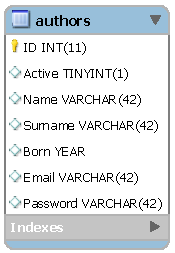
\includegraphics[scale=1.4]{obrazky-figures/authors.pdf}
    \caption{Atributy tabulky \textit{authors}, použité pro demonstraci SQLi}
\end{figure}

Hesla jsou záměrně ukládána v~otevřené podobě (tzv. \textit{plaintextu}), což umožňuje nejen jejich vypsání vlastníkům na základě filtrování dle 
\textit{ID}, ale také daleko jednoduší prozrazení informací neautorizovanému uživateli. Pokud útočník najde způsob, jak se dostat k~záznamům 
z~databáze, nemusí se už dále ani snažit --- znění přihlašovacích údajů má naservírované na stříbrném talíři. I~proto je velmi důležité, aby byla 
hesla ukládána v~šifrované podobě. Protože však toto téma již přesahuje zadání diplomové práce, zvědavý čtenář nechť si například přečte diskuzi 
ohledně možností bezpečného ukládání hesel na \textit{Information Security Stack 
Exchange}\footnote{\url{security.stackexchange.com/questions/211/how-to-securely-hash-passwords}}. \\

Ponecháme-li stranou neexistující zabezpečení uložených hesel, budeme se nyní zabývat otázkou, zda se případný útočník může dostat k~údajům patřící
jinému uživateli, než je on sám (pokud je vůbec přihlášen), či dokonce ke kompletní databázi uživatelů. \\

\Bat{} Začneme s~obsahem tabulky \ref{fig:data_authors}, tak jak si jej legitimně může prohlédnout například \mbox{uživatel} \textit{root},
ale již by neměl být spatřen neautorizovanou osobou:

\begin{lstlisting}[language=sql]
MariaDB [sqli-prevention]> SELECT * FROM authors;
\end{lstlisting}

\begin{figure}[h!]
    \label{fig:data_authors}
    \centering
    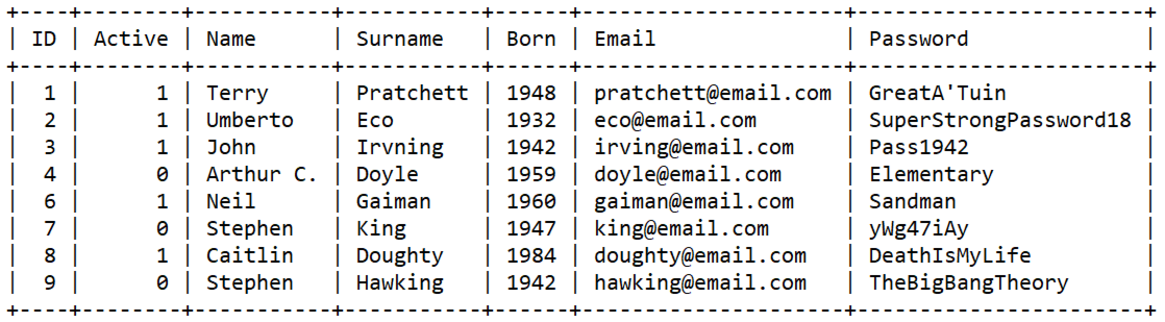
\includegraphics[scale=0.75]{obrazky-figures/table.pdf}
    \caption{Kompletní výpis dat z~tabulky \textit{authors}}
\end{figure}

\Bat{} Celý výpis tedy není chtěným cílem a obecný dotaz \texttt{SELECT * FROM authors;} tedy pravděpodobně nevyužijeme. Můžeme ale předpokládat
například dotaz \texttt{SELECT Name,\\Surname,Email,Password FROM authors WHERE ID = *** AND Active = 1;}, kde bude na místo \texttt{***}
vložen vstup od uživatele. Pokud uživatel zadá číslo \texttt{1}, výstup bude následující:

\begin{lstlisting}[language=sql]
MariaDB [sqli-prevention]> SELECT Name, Surname, Email, Password 
                           FROM authors WHERE ID = 1 AND Active = 1;
+-------+-----------+---------------------+-------------+
| Name  | Surname   | Email               | Password    |
+-------+-----------+---------------------+-------------+
| Terry | Pratchett | pratchett@email.com | GreatA'Tuin |
+-------+-----------+---------------------+-------------+
1 row in set (0.00 sec)
\end{lstlisting}

\Bat{} Co se ale stane v~případě, pokud uživatel nezadá pouze číslo? Jaký následek bude mít vstup \texttt{1 OR 1 = 1; -{}- }?

\begin{lstlisting}[language=sql]
MariaDB [sqli-prevention]> SELECT Name, Surname, Email, Password 
                           FROM authors WHERE ID = 1 OR 1 = 1; 
                           -- AND Active = 1;
+-----------+-----------+---------------------+-----------------------+
| Name      | Surname   | Email               | Password              |
+-----------+-----------+---------------------+-----------------------+
| Terry     | Pratchett | pratchett@email.com | GreatA'Tuin           |
| Umberto   | Eco       | eco@email.com       | SuperStrongPassword18 |
| John      | Irvning   | irving@email.com    | Pass1942              |
| Arthur C. | Doyle     | doyle@email.com     | Elementary            |
| Neil      | Gaiman    | gaiman@email.com    | Sandman               |
| Stephen   | King      | king@email.com      | yWg47iAy              |
| Caitlin   | Doughty   | doughty@email.com   | DeathIsMyLife         |
| Stephen   | Hawking   | hawking@email.com   | TheBigBangTheory      |
+-----------+-----------+---------------------+-----------------------+
8 rows in set (0.00 sec)
\end{lstlisting}

Útočník se nám právě dostal ke všem záznamům a to dokonce i k~těm, které značí neaktivní uživatele a neměli by být vypisování vůbec.
Jak je to možné? SQL dotaz zde byl vyhodnocen následovně --- nejdříve jsme, jako v~minulém případě, požádali o~všechny záznamy, kde
se hodnota ID rovná 1. Příkaz poté ale pokračuje a to logickým operátorem \texttt{OR}. Protože výraz \texttt{1 = 1} je vždy pravdivý,
celá podmínka se vyhodnotí také jako pravdivá ve všech případech, i pokud ID není rovno jedné. Útočník navíc chytře zakomentoval
zbytek původního dotazu, aby vyloučil další případné podmínky, či příkazy. Tímto poměrně jednoduchým způsobem jsme si vynutili
vrácení kompletně všech záznamů z~dané tabulky.\\

\Bat{} Obdobným způsobem lze rovněž přidávat vlastní příkazy, které mohou vést k~vyzrazení dalších informací, nebo dokonce k~jejich úpravě,
či smazání. Původní dotaz tak může být pozměněn třeba na 
\texttt{SELECT Name, Surname, Email, Password FROM authors WHERE ID = 2; DROP TABLE authors; -{}- AND Active = 1;},
díky čemuž rázem přicházíme o~veškerá data i se strukturou tabulky.

\begin{lstlisting}[language=sql]
/* Příkaz pro výpis všech tabulek v databázi */
MariaDB [sqli-prevention]> SHOW TABLES;
+---------------------------+
| Tables_in_sqli-prevention |
+---------------------------+
| authors                   |
+---------------------------+
1 row in set (0.00 sec)

MariaDB [sqli-prevention]> SELECT Name, Surname, Email, Password 
                           FROM authors WHERE ID = 2; DROP TABLE authors; 
                           -- AND Active = 1;



+---------+---------+---------------+-----------------------+
| Name    | Surname | Email         | Password              |
+---------+---------+---------------+-----------------------+
| Umberto | Eco     | eco@email.com | SuperStrongPassword18 |
+---------+---------+---------------+-----------------------+
1 row in set (0.00 sec)

Query OK, 0 rows affected (0.28 sec)

/* Předchozí dotaz smazal celou tabulku */
MariaDB [sqli-prevention]> show tables;
Empty set (0.00 sec)
\end{lstlisting}

Na příkladu výše je rovněž vidět další dotaz, který je pro útočníka lákavým. Díky příkazům typu \texttt{SHOW TABLES;}, nebo
\texttt{SHOW DATABASES;} získává přehled o~struktuře tabulek, či databází, čehož následně může využít při dalších útocích. \\

Již Forristal\footnote{\url{phrack.org/issues/54/8.html}} upozorňoval, že situaci sice útočníkovi mírně zkomplikujeme,
pokud jeho vstup budeme uvozovat \texttt{SELECT * FROM authors WHERE ID='***' AND Active = 1;} a~tudíž se jeho vstup bude vyhodnocovat jako řetězec,
ale i to lze obejít poměrně jednoduše. Útočníkovi stačí zadat například \texttt{SELECT * FROM authors WHERE ID='' OR 1=1; -{}- ' AND \\ Active = 1;}
a získává stejný výsledek. \\

Na závěr této podkapitoly si nelze nedovolit ještě jednu drobnou poznámku z~pohledu bezpečnosti. Kromě prvního příkladu jsme
v~dalších dotazech měli explicitně zvolené atributy, které jsme chtěli vracet. Použití \texttt{SELECT * \dots} je sice
velmi lákavé, avšak toto řešení není zcela vhodné. O~nevýhodách tohoto na první pohled bezpečného SQL dotazu píše například Ryan Flynn na svém 
blogu\footnote{\url{www.parseerror.com/blog/select-*-is-evil/}}, kde se dočteme, jak je výběr všech sloupců nejen proti dobrým praktikám 
programátora, protože znepřehledňuje a zatemňuje kód při dlouhodobém vývoji, ale rovněž může výrazně zvyšovat paměťové nároky aplikace. 

\subsection{Existující obrana proti SQL injection}\label{subsec:3:tools}
Jak jsme si uvedli v části \ref{subsec:3:sqlihistorie}, SQL injection útok není žádnou novinkou, přesto je přetrvávajícím problémem. 
Není to však z důvodu nedostatečné snahy vytvářet prostředky ochraňující před touto zranitelností, ve skutečnosti existuje celé množství 
řešení, s různou mírou úspěšnosti a zabezpečení. Zde si v krátkosti uvedeme jen některé z nich, především proto, že si tato práce ani neklade za cíl 
poskytnout vyčerpávající přehled všech dostupných nástrojů. Rozšiřující informace lze pak nelézt například na stránkách komunity 
\textit{OWASP}\footnote{\url{www.owasp.org}}. \\

\Bat{} \textbf{mysql\_real\_escape\_string} \\
Začneme metodou, jejíž používání se už delší dobu oficiálně nedoporučuje\footnote{\url{php.net/manual/en/function.mysql-real-escape-string.php}},
především z~důvodu, že již není součástí aktivního vývoje, přesto díky internetu stále přežívá, především v~rámci diskuzních fór a starých blogových příspěvků, 
kde je často označována jako bezpečná.
\newpage
Metoda vkládá před speciální znaky ($\textbackslash x00$, $\textbackslash n$, $\textbackslash r$, $\textbackslash \textbackslash$, 
\texttt{'}, $"$, $\textbackslash x1a$) zpětné lomítko, provádí tedy tzv. escapování (\textit{escape}). To zabraňuje situaci, kdy útočník předčasně 
ukončí uvozenou část pro svůj vstup a přidává následně své dotazy, jak jsme si uvedli výše. Z příkladu 
\texttt{SELECT * FROM authors WHERE ID=' ' OR 1=1; -{}- ' AND Active = 1;} by se tedy stal neškodný dotaz 
\texttt{SELECT * FROM authors WHERE ID='$\textbackslash$' OR 1=1; -{}- ' AND Active = 1;}, kdy je celý vstup od uživatele vyhodnocen 
jako řetězec. \\ 

Tento přístup však funguje pouze za předpokladu, že je uživatelský vstup vkládán do jednoduchých uvozovek. Přestože tímto způsobem lze vkládat
i celočíselné hodnoty, které jsou následně správně přetypovány, je zde jedna výjimka --- pokud chceme zadávat hodnotu LIMIT, je nejdříve nutné převést
vstup na celočíselnou hodnotu, jinak bude dotaz zamítnut. \\

Co je ale podstatnější, existují způsoby, jak tuto funkci 
obejít\footnote{\url{stackoverflow.com/questions/5741187/sql-injection-that-gets-around-mysql-real-escape-string}}. 
První cílí na rozdílné nastavení znakové sady na straně klienta a na straně serveru, díky kterým funkce nerozezná všechny speciální znaky,
které však server již vyhodnotí správně. Další využívají volby \texttt{NO\_BACKSLASH\_ESCAPES}, která zakazuje escapování,
což z podstaty znemožňuje správnou úpravu vstupu. \\

Nástupce této funkce, \texttt{mysqli\_real\_escape\_string}\footnote{\url{php.net/manual/en/mysqli.real-escape-string.php}}, sice slibuje lepší práci se znakovými sadami, 
přesto je náchylná na obdobné problémy a v další kapitole si blíže vysvětlíme důvody, proč z podstaty problému nemůže být stoprocentní ochranou proti SQLi kvůli 
nedostatečným principům ošetřování vstupů. \\

\Bat{} \textbf{PDO}\\
V současné době je nejvíce doporučováno PDO (\textit{PHP Data Objects}), poskytující rozhraní pro práci s databázemi v jazyce PHP (existují obdobné
implementace i pro jiné jazyky). Výhoda je především v podpoře předzpracovaných příkazů (\textit{prepared statements}), které umožňují zpracovat SQL dotaz 
pouze jednou a následně jej opakovaně spouštět se stejnými i různými parametry\footnote{\url{php.net/manual/en/pdo.prepared-statements.php}}. 
Při použití s vázanými proměnnými (\textit{bind variables}), je umožněné bezpečné provedení dotazu přes případnou přítomnost SQLi, protože dopředu
omezíme, jak má být vstup interpretován, ku příkladu jako řetězec, bez ohledu na uzavírající uvozovky. Tento přístup se jeví jako bezpečný,
přestože může mít občasně vliv na výkon aplikace \cite{OWASP2018}.\\

\Bat{} \textbf{Ošetření vstupu pomocí White listu}\\
Poslední metoda se zaměřuje více na obsah uživatelského vstupu, než jeho strukturu a je založen na myšlence, že existuje množina slov, kterou
od uživatele nepřijmeme v žádné situaci. Může se jednat o názvy tabulek a sloupců, nebo určení pořadí řazení, které pro nás detekuji SQLi. 
V případě, že přeci jen potřebujeme povolit některé z výše uvedených, využije se tzv. \textit{white list} množiny \cite{OWASP2018}, která určí povolené výjimky, 
například s jakými tabulkami uživatel může pracovat, nebo že může řadit pouze pomocí klíčových slov \texttt{ASC} a~\texttt{DESC}.

\section{Další příklady útoků} \label{sec:3:attacks}
Kromě SQLi, popsaného v předchozí podkapitole, tady zmíníme ještě jeden útok, který rovněž spadá do kategorie zranitelností, zaměřující se
na nedostatky při zpracování vstupu. Liší se však od injection útoků, kdy útočník mění syntax i sémantiku například SQL dotazů, či URL
adresy a místo toho využívá různé \textit{interpretace} stejného vstupu. Řeč je o~zranitelnostech ve standardu \textit{X.509}.

\subsection{X.509} \label{subsec:3:x509}
Již jsme zmínili, že jedním z~prostředků, jak zvyšovat bezpečnost, je použití autentizace, tedy ověřování identity. Jak ale provést něco takového 
na internetu, který je ze své podstaty anonymní? Jak si můžeme být jisti, že komunikujeme s~osobou, či systémem, který je skutečně tím, za co se vydává? \\

Běžně se používá kryptografie a elektronické podpisy, ale ty neřeší, kdo je majitelem privátního klíče. Proto používáme certifikáty veřejných klíčů, 
což jsou datové struktury, které váží veřejné klíče k~subjektům. Tento certifikát je pak podepsán certifikační autoritou 
(\textit{certification authority -- CA}) \cite[str. 9-10]{RFC:X509}. \\

X.509 je standard popisující formát certifikátu, v~současné době používaný ve verzi 3. \mbox{Využívají} jej lidé, ale i procesy, které používají 
klientský software a jsou subjekty uvedených v~certifikátech. Mezi ně patří uživatelé elektronické pošty, klienti webových prohlížečů, webové 
servery a další \cite[str. 9-10]{RFC:X509}. X.509 nespecifikuje pouze formát certifikátů, ale i seznam zrušených certifikátů 
(\textit{certificate revocation list -- CRL}), parametry certifikátů a~metody kontroly platnosti certifikátů \cite[str. 130]{Slovnik2015}. \\

Jak a v~čem se projevují zranitelnosti standardu X.509? Jak uvádí článek \textit{PKI Layer Cake: New Collision Attacks Against the Global X.509 Infrastructure} 
\cite[str. 1]{Kaminsky2010}, je zde vícero kategorií, přičemž zmíníme především jednu, která dokazuje, proč je důležité, aby každé zpracování vstupních
dat probíhalo ekvivalentním způsobem. \\

Pokud žádáme o~certifikát, zadáváme tzv. \textit{commom name} (CN), pod kterým je daný subjekt znám, 
například adresu \url{www.paypal.com}. V~X.509 však docházelo k~nežádoucím stavům, kdy CA vydávalo certifikáty neautorizovaným jménům. 
Útočník pak mohl požádat o~certifikát na adresu ve tvaru \url{www.paypal.com\\0.evil.com}, kterou ale některé webové prohlížeče interpretovaly 
pouze jako \url{www.paypal.com\\0}. \\

Stejně tak se lišila implementace v~případě, že útočník zadal vícero jmen, ku příkladu \url{CN=www.paypal.com/CN=www.evil.com}, kdy v~některých 
případech bylo bráno v~potaz pouze první jméno, jindy poslední. Tyto případy jsou již naštěstí opraveny, ale jsou krásnými příklady zranitelností, 
které se problematicky testují, ale lze jim předejít již v~době návrhu, kdyby bylo dodrženo zásad LangSecu, jak si uvedeme v~následující kapitole.\\

%%%%%%%%%%%%%%%%%%%%%%%%%%%%%%%%%%%%%%%%%%%%%%%%%%%%%%%%%%%%%%%%%%%%%%%%%%%%%%%%%%%%%%%%%%%%%%%%%%%%%%%%%%%%%%%%%%%%%%%%%%%%%%%%%%%%%%%%%%%%%%%%%%%%%
% 4. Kapitola
%%%%%%%%%%%%%%%%%%%%%%%%%%%%%%%%%%%%%%%%%%%%%%%%%%%%%%%%%%%%%%%%%%%%%%%%%%%%%%%%%%%%%%%%%%%%%%%%%%%%%%%%%%%%%%%%%%%%%%%%%%%%%%%%%%%%%%%%%%%%%%%%%%%%%
\chapter{LangSec}\label{ch:langsec}
Po obsáhlejším úvodu, zahrnujícím seznámení s~teorií formálních jazyků \ref{ch:theory} a bezpečností \ref{ch:security}, tak jak ji chápeme ve světě 
informačních technologií, si nyní vysvětlíme, jak a především proč by měla mít teorie formálních jazyků zásadní slovo při tvorbě bezpečných systémů. \\

Primárními zdroji pro tuto kapitolu se staly článek Security Applications of Formal Language Theory \cite{Sass2013} publikovaný v~roce 2013 v~IEEE 
Systems Journal, jeho starší verze v~podobě technické zprávy \cite{Sass2011} a oficiální webové stránky projektu LangSec \cite{LangSecWeb}. \\

Nutno ještě podotknout, že pojmu systémy budeme užívat v~obecném slova smyslu bez striktní definice a zvlášť v~této kapitole může představovat 
síťový protokol, obecně software, ale i celý operační systém. Autoři dokonce v~technické zprávě z~roku 2011 \cite[str. 23]{Sass2011} naznačují, 
že základní principy, které představují, mohou být (a možná by měly být) aplikovány i na hardware. \\

Co se tedy skrývá pod názvem LangSec? A~co nového přináší do problematiky bezpečnosti? \\

LangSec, neboli Language-Theoretic Security, je přístup, který se snaží reflektovat ne příliš optimistickou situaci, která vládne na internetu kolem 
bezpečnosti a kterou jsme nastínili již v~úvodní části. Avšak, na rozdíl od populárního názoru, že za všudypřítomnými zranitelnostmi stojí 
nedostatečná snaha programátorů testovat a opravovat svoji práci, autoři přístupu LangSec vidí zdroj problému již v~základních principech, 
podle kterých systémy vytváříme. \\

Jako klíčový problém uvádí přístup ke zpracování vstupů, které je často řešeno ad-hoc implementací \cite{LangSecWeb}. Přitom informace, které systém
dostává ze vstupu jsou z~podstaty nedůvěryhodné a je nutné k~nim takto přistupovat. Pokud má systém odlišit validní vstup od škodlivého, může k~němu
přistupovat jako k~formálnímu jazyku, jehož zpracování znamená jeho rozpoznání. To však znamená, že program musí mít právě ekvivalentní výpočetní 
sílu jako rozpoznávaný jazyk (proč není vhodné využívat programů s~větší výpočetní silou, si vysvětlíme později). \\

Pokud pak vezmeme v~potaz komplexní jazyky, z~úplného rozpoznání platných nebo očekávaných vstupů se stává nerozhodnutelný problém. Programátoři 
i testeři se mohou snažit, jak chtějí. Na světě není dostatek testů, které by zajistily bezpečnost takových programů. Mnoho populárních protokolů 
a formátů narazilo na tento problém, což je empirický fakt \cite{LangSecWeb}. \\

I~Dan Geer \cite{Geer2010} upozorňuje, že potíže se zabezpečením internetu, který nám začíná přerůstat přes hlavu, spočívá v~samotných základech, 
na kterých byl tento ekosystém postaven. 
\textit{\uv{Be conservative in what you do, be liberal in what you accept from others}}, tak zní Postelův princip robustnosti ze specifikace TCP, 
který byl široce akceptován jako základní princip implementace protokolů.  Geer s~tím ale nesouhlasí a tvrdí, že lepší a bezpečnější radou je úprava 
na \textit{\uv{be conservative in what you accept}} \cite[str. 3]{Geer2010}. \\

V~dalších částech této kapitoly si ještě podrobněji vysvětlíme vážnost důsledků, které nastávají, pokud je systém navržen bez ohledu na výpočetní 
sílu jazyka. Předtím si ale představíme filozofii LangSecu pomocí několika sloganů, které nám pomohou lépe pochopit klíčové aspekty tohoto 
přístupu \cite{LangSecWeb} a které slibují zlepšení bezpečnosti i rozsáhlých systémů a protokolů \cite[str. 489]{Sass2013}. \\

\textbf{Úplné rozpoznání před zpracováním} (\textit{Full recognition before processing}) -- každý program, který přijímá vstup jej vlastně 
rozpoznává. Měl by tedy přijímat pouze validní, či očekávané vstupy a zamítat ty chybné, či potenciálně škodlivé. V~praxi je však rozeznávání 
implementováno ad-hoc metodou a rozprostřeno skrz celý program, což může vést k~nedostatečné ochraně a k~náchylnostem na zranitelnosti. \\

\textbf{Snižujme nenasytnost po výpočetní síle} (\textit{Reduce compiting power greed}) -- v~jednoduchosti je krása, ale také bezpečnost, jak tvrdí 
LangSec. Výpočetní výkon v~kódu nemusí být pouze zbytečný, může být otevřenou branou pro útočníky. Proto bychom se měli pracovat na snižování 
výpočetních nároků protokolů. \\

\textbf{Zastavme podivné stroje} (\textit{Stop weird machines}) -- pokud pracujeme s~komplexním protokolem, potřebujeme i analyzátor odpovídající 
síly. Ten se však velmi lehce může proměnit ve \textit{weird machine} (výpočetní prostředí uvnitř našeho systému, na kterém běží škodlivý výpočet 
útočníka \ref{app:a:weirdmachine}), otevřený pro útoky. Proti této hrozbě má LangSec cíl -- nechť jsou naše protokoly bezkontextové, či regulární. \\

\textbf{Ne! turingovsky úplným jazykům} (\textit{No more Turing-Complete Input Languages})  -- jazyky, které jsou turingovsky úplné 
představují pro bezpečnost velkou hrozbu, protože problém jejich rozpoznávání je nerozhodnutelný. Nezáleží, kolik testů a oprav vývojáři provedou. 
Protokoly a formáty souborů založené na takových jazycích nebudou nikdy opravdu bezpečné. \\

\textbf{Výpočetní ekvivalence pro všechny koncové body protokolů} (\textit{Computional Equivalence fot all protocol endpoints}) -- při komunikaci 
je potřeba, aby obě strany, jak odesilatel, tak příjemce, interpretovaly zprávu stejně. To znamená výpočetně ekvivalentní analyzátory, což je ale 
již od nedeterministických bezkontextové gramatiky nerozhodnutelný problém. \\

Není nic překvapivého na tom, že na zabezpečení systémů bychom měli myslet již ve fázi návrhu. Autoři však přinášení oporu při této fázi, která 
eliminuje chyby, jenž by v~důsledku nerozhodnutelných problémů nebyly odstranitelné s~pomocí klasického testování a~opravování chyb. Přesto zde máme 
mnoho praktických systémů, které nebyly navrženy ani vytvořeny s~ohledem na bezpečnost. Takové systémy ale nemusíme hned zavrhnout, spíše by se mělo 
pracovat na jejich vylepšení \cite[str. 489]{Sass2013}.

\section{Systémy a modularita} \label{sec:4:systems}
V~běžné praxi málokdy nastává situace, kdy by systém vytvářel jediný člověk. Projekty rychle rostou do rozměrů, kdy není v~lidských silách a časových 
možnostech implementovat vše samostatně od úplného začátku. I~proto považujeme modularitu, kdy je systém složen z~komponent (často od jiných autorů), 
jakou samozřejmý a možná jediný rozumný způsob vytváření složitějších systémů, bez něhož by byl celý proces \uv{nepoddajný} \cite[str. 489]{Sass2013}. \\

Je ale takové řešení bezpečné? Lze skládat komponenty tak, abychom nenarušili bezpečnost systému? Jak částečně odhalily slogany na začátku kapitoly, 
i zde se skrývá možný zdroj nežádoucích zranitelností. V~modulárních systémech mezi sebou jednotlivé části komunikují pomocí zpráv, které však musíme 
řešit se stejnou opatrností, jako se vstupy. Pro zajištění bezpečnosti proto potřebujeme lepšího výpočetně-teoretického chápání těchto interakcí. 
Našimi cíli je kontrola vstupu v~každé komponentě a identická interpretace zpráv přenášena mezi komponentami pro všechny koncové 
body \cite[str. 489]{Sass2013}. \\

Nejdříve se ale podívejme na bezpečnost z~pohledu jedné komponenty.  Každá komponenta musí být schopna přijímat vstupy nebo zprávy přes jedno nebo více 
rozhraní. To však vytváří \textit{attack surface} \ref{app:a:attacksurface}, což je kód, který může být spuštěn neautorizovanými uživateli, a~kterého 
využívá velká část útoků. Český ekvivalent tohoto pojmu se ve Výkladovém slovníku kybernetické bezpečnosti neuvádí a proto tento termín nebude přeložen 
ani zde. Komponenta rovněž musí být schopna odmítnou vstup bez toho, aniž by ztratila integritu, nebo se dostala do neočekávaného 
stavu \cite[str. 490]{Sass2013}. \\

Pokud pak řešíme bezpečnost jako celek více navzájem komunikujících komponent, potřebujeme, aby byly zasílané zprávy vnímané identicky. Avšak jak říká 
známé latinské přísloví: \textit{\uv{Duo cum faciunt idem, non est idem}} --- když dva dělají totéž, není to totéž. I~zde se projeví problém 
nerozhodnutelnosti, protože pokud bychom chtěli formálně dokázat, že nás systém zpracovává zprávy stejným způsobem, řešíme otázku ekvivalence gramatik, 
což je nadlidský úkol pro gramatiky silnější než deterministicky bezkontextové. \\ 

Na první pohled banálně vypadající problém odlišné implementace může znamenat vznik kritických zranitelností, jak bylo ukázáno na 
X.509 (\ref{subsec:3:x509}) a ASN.1. \\

Dalším příkladem selhání komunikace mezi komponentami představuje útok \textit{SQL injection} \ref{app:a:sqlinjection}, kdy útočník předkládá databázi 
vstupní dotaz, který je platný pro databázi v~izolaci, ale neplatný v~kontextu role databáze ve větší aplikaci \cite[str. 491]{Sass2013}.

\section{Bezpečnost systému} \label{sec:4:systemsecurity} 
Pokud mluvíme o~bezpečnosti systému a způsobech, jak ji zajistit, nestačí pouze diskutovat kroky a postupy jeho návrhu a tvorby. Nestačí nám víra, že 
pokud dodržíme určitý postup, budou naše programy rázem bez chyb a zranitelností. Proto se snažíme najít způsoby, jak dokázat, že nás systém pracuje tak, 
jak jsme zamýšleli a že je tudíž bezpečný. \\

Pro tyto účely se používají dva druhy důkazů: formální a neformální. Formální důkaz je založen na přesném a detailním formálním systému, který může být 
zkontrolován počítačem. Neformální důkaz je naproti tomu dostatečně přesný na to, aby přesvědčil inteligentního, skeptického člověka a obvykle se 
provádí ve stylu \uv{deníku matematických důkazů} \cite[str. 125]{Lamport1977}. \\

Při prokázání správnosti programu nahlížíme na dvě z~podstaty rozdílné typy vlastností, které označujeme jako bezpečnost (safety) a živost (liveness). 
Bezpečnost značí, že se něco nestane. Například, pokud program dostane správný vstup, nemůže zastavit, pokud nevyprodukuje správný výstup. Naproti tomu 
živost představuje něco, co se musí stát. Například, tvrzení, že program zastaví, pokud je jeho vstup správný \cite[str. 125]{Lamport1977}. \\

Ověřování programu je ovšem v~obecném případě nerozhodnutelné, a přestože se vyvíjí mnoho nástrojů pro verifikaci založených na různých přístupech, 
problémy se škálovatelností a úplností algoritmického ověřování zabránily, aby formální přístup nahradil testování a audity kódu jako průmyslový 
standard pro zajištění kvality softwaru \cite[str. 490]{Sass2013}. \\

Analyzátory také vykazují určité vlastnosti bezpečnostní a živosti. Mezi bezpečnostní vlastnosti řadíme i spolehlivost (\textit{soundness}), 
tedy že analyzátor přijme řetězce pouze z~daného jazyka a vše ostatní odmítne. Obecně spolehlivost označuje dokázané tvrzení, že systém pracuje 
ve shodě s~danou specifikací. Další bezpečnostní vlastností je ukončení (\textit{termination}), jistota, že analyzátor vždy zastaví. 
Mezi vlastnosti živosti se řadí úplnost (\textit{completenes}), tedy že analyzátor přijímá všechny řetězce daného jazyka \cite[str. 490]{Sass2013}.

\section{Kontrola vstupu jako klíčový aspekt bezpečnosti} \label{sec:4:inputcontrol}
Každá komponenta systému přijímá vstupní zprávy. Zdroj se může různit – odesilatelem může být například uživatel, jiná komponenta v~rámci systému, 
či dokonce mimo něj. To, zda je implementace komponenty správná a bezpečná úzce souvisí s~tím, jak je tento vstup  analyzován, ať z~pohledu syntaxe, 
tak sémantiky. \\

Programy, které implementují protokoly s~jednoznačným vstupním jazykem mohou a měly by být plně rozpoznatelné 
\cite[str. 490]{Sass2013}. Příkladem mohou být  souborové formáty, kódování, skriptovací jazyky, síťové a bezpečnostní protokoly. \\

Bohužel, v~praxi se stále nejčastěji spoléhá na ad-hoc analyzátory bez ohledu na jejich rozpoznávací sílu, což narušuje bezpečnost a vede k~mnoha 
zranitelnostem \cite[str. 490]{Sass2013}. Přitom pro formální analýzu na kontrolu vstupu se dají se použít knihovny, či nástroje pro generování 
kódu --- máme prokazatelně správné kombinátory analyzátorů a generátory se zárukou zastavení \cite[str. 490]{Sass2013}. \\

Jak jsme uvedli v~kapitole \ref{ch:theory}, klasifikace podle Noama Chomského rozděluje gramatiky do hierarchie dle vyjadřovací síly, která koreluje 
s~komplexností automatu, který přijímá jazyky vytvořené těmito gramatikami. Pro formální validaci vstupu tedy vyžadujeme automat (respektive analyzátor) 
minimálně tak silný jakým je vstupní jazyk. \\

Kromě minimální síly je zde ale i požadavek, aby analyzátor nebyl zbytečně silnější, než je nutné.
W3C pravidlo nejmenší síly (Rule of Least Power) \cite{w3cpower} nám říká, že máme užívejme nejslabší jazyk vhodný pro vyjádření informací, 
omezení a programů na webu. Kromě výpočetní síly, kterou dáváme všanc útočníkovi je zde i hrozba plynoucí z~vlastností jazyků. Pokud bychom 
například měli rekurzivně vyčíslitelný jazyk, zpracování škodlivého kódu může způsobit, že analyzátor selže v~zastavení a bude donekonečna cyklit. \\ 

V~technické zprávě z~roku 2011 \cite[str. 22]{Sass2011} Sassaman a spol. píší, že analyzátor, který přesahuje sílu vstupu, by měl být považován za 
rozbitý. Jakákoliv zvýšení síly vstupního jazyka by pak mělo být považováno za udělení dalšího oprávnění a tedy i zvýšení bezpečnostních rizik. \\

Mimo zvýšení bezpečnosti W3C upozorňuje i na skutečnost, že vyjádření vazeb, vztahů a pokynů pro zpracování v~méně výkonných jazycích zvyšuje 
flexibilitu, s~jakou mohou být informace znovu použity. Jazyk je vhodné volit i s~ohledem na snadnost (či obtížnost) analýzy, přičemž W3C zde 
v~některých případech upřednostňuje funkcionální jazyky před jejich imperativními ekvivalenty \cite{w3cpower}. \\

W3C na závěr ještě doporučuje jiný přístup a to vytvářet škálovatelné rodiny jazyků s~pojmenovanými podmnožinami a rozšířenějšími verzemi, 
které jsou schopnější, ale také obtížnější na analýzu. Příkladem může být jazyk OWL Web Ontology, jenž je nabízen ve třech variantách rostoucího 
výkonu: OWL Lite, OWL DL a OWL Full. Standardizace podmnožin jazyka může usnadnit jednoduché modely pro publikování na webu a zároveň zajistit 
integraci s~výkonnějšími jazykovými variantami v~případě potřeby \cite{w3cpower}. \\

Nutno podotknout, že ne vždy se nový vývoj řídí těmito doporučeními. Současná verze HTML5 je ve společnosti CSS turingovsky úplná, 
přestože HTML4 nebyla \cite[str. 22]{Sass2011}.

\section{Zneužití jako neočekávaná komunikace} \label{sec:4:exploits}
\textit{Exploit} \ref{app:a:exploit}, česky zneužití, je chyba, kód, či bezpečnostní díra, kterou může využít útočník k~tomu, aby v~systému prováděl 
neočekávané nebo neautorizované výpočty \cite[str. 135]{Slovnik2015}. Jedná se tedy o~situaci, kdy se systém dostane do stavu, který nebyl zamýšlen 
jeho autory. Může pak například vyzradit citlivé údaje, modifikovat je, či umožnit útočníkovi zadávat příkazy, na které by v~normální situaci neměl 
oprávnění. Kdy a jak ale vzniká takové zneužití? \\

Systém, kterému jsou zaslány z~zvenčí zprávy (například protokolové povahy), přijímá požadavek, aby provedl výpočet na nedůvěryhodném vstupu. 
Tuto skutečnost můžeme popsat i tak, že přijímá zprávu M, která je kódována odesilatelem, značeno E(M). Dekóduje tuto zprávu, tedy provede operaci 
D(E(M)) a následně vykoná sekvenci operací v~závislosti na získaném výsledku procesu dekódování \cite[str. 492]{Sass2013}:
\vspace*{\baselineskip}
\begin{center}  
$E(M) \rightarrow D(E(M)) * C(D(E(M))) $
\end{center}
\vspace*{\baselineskip}
To samo o~sobě by nikdy nemělo vést ke spuštění škodlivému kódu či neautorizovanému zveřejnění citlivých dat, přesto je podvrhnutí vstupu stále 
nejúspěšnější metoda útoků \cite[str. 492]{Sass2013}. Jedná se de facto o~povolenou, avšak již ne očekávanou akci. Proto už ve fázi návrhu 
musíme stanovit předpoklady pro popis platného vstupu. 

%%%%%%%%%%%%%%%%%%%%%%%%%%%%%%%%%%%%%%%%%%%%%%%%%%%%%%%%%%%%%%%%%%%%%%%%%%%%%%%%%%%%%%%%%%%%%%%%%%%%%%%%%%%%%%%%%%%%%%%%%%%%%%%%%%%%%%%%%%%%%%%%%%%%%
% 5. Kapitola
%%%%%%%%%%%%%%%%%%%%%%%%%%%%%%%%%%%%%%%%%%%%%%%%%%%%%%%%%%%%%%%%%%%%%%%%%%%%%%%%%%%%%%%%%%%%%%%%%%%%%%%%%%%%%%%%%%%%%%%%%%%%%%%%%%%%%%%%%%%%%%%%%%%%%

\chapter{LangSec v~praxi} \label{ch:langsecapp}
V~předchozí kapitole jsme rozebírali především teoretickou podstatu filosofie LangSecu, ale jak tedy máme postupovat při návrhu a tvorbě systémů
a především, čemu se máme pokusit vyhnout? Jak jsme si již uvedli, LangSec klade důraz na správné zpracovávání a interpretaci vstupu, na jejichž 
nedostatky cílí převažující část chyb a zranitelností současné doby.

\section{Praktická doporučení} \label{sec:5:dosanddonts}

\textbf{Ad-hoc zpracování vstupu} \\
Vágní popis vstupních dat nejen komplikuje jejich rozpoznávání, ale i verifikaci.
Místo toho je tedy nejdříve důležité pracovat s~popisem platných vstupních dat jako s~formálním jazykem, ať už přijímáme pakety, či zprávy, nebo 
například url adresu. Součástí tohoto kroku je také snaha minimalizovat sílu jazyka, protože jak jsme uvedli výše, čím větší je vyjadřovací síla 
jazyka, tím obtížnější je jeho rozpoznávání a pokud překročí hranici turingovsky-úplného jazyka, z~rozeznávání vstupu se stává nerozhodnutelný 
problém. \\

\textbf{Rozdíly v~parsování} \\
Různá interpretace vstupních dat podle komponent porušují bezpečnost, protože přináší nekonzistentní stavy a neočekávané výpočty. Příklad může být 
již popsaný případ zranitelnosti X.509 z~části \ref{subsec:3:x509}, kdy byl podepsaný certifikát interpretován jinak certifikační autoritou a~jinak webovým 
klientem. Znovu si také připomeňme, že problém stejného zpracování je vlastně otázka ekvivalence jazyků a nad třídu deterministicky bezkontextových 
gramatik je to nerozhodnutelný problém. V~shrnujícím dokumentu \cite{LangSecBof} se doporučují vyhýbat vstupním jazykům a systémům, jejichž 
důvěryhodnost je založena na rovnocennosti parsovacích komponent. \\

\textbf{Mísení rozpoznání a zpracování vstupu} \\
Tzv. \uv{shotgun parser}, jak jej označují autoři LangSecu, značí smíšené základní ověřování vstupu a logicky následné kroky zpracování,
které se objevují až po rozpoznání celé zprávy. 
LangSec v~dokumentu \cite{LangSecBof} doporučuje nejdříve plně rozpoznávat vstupní jazyk, kdy již v~tomto kroku odmítneme nevyhovující vstupy a ty
vyhovující transformujeme na požadované strukturované údaje. Samotné zpracování pak probíhá nad datovými strukturami, ne však nad surovými daty. \\

\textbf{Přidávání nových vlastností} \\
Přidávání nových vlastností je vždy výzva, ať už s~použitím LangSecu, nebo bez něj. Vývojář by měl vždy dobře zvážit důsledky změn na bezpečnost,
především pokud by změny měly vést ke zvýšení požadované výpočetní síly. Je silně doporučováno zachovávat stejnou třídu vstupního jazyka. 

\section{Nástroje} \label{sec:5:tools}
LangSec vzbudil mezi odbornou veřejností velký ohlas. 
Svědčí o~tom například i již čtyři ročníky LangSec Workshopů na \textit{IEEE Symposium on Security \& Privacy Workshops}, konaných od roku 2014 
v~Kalifornii, na kterých se podíleli například Doug McIlroy, Dan Geer, Caspar Bowden a mnozí další. V~roce 2017 Perry Metzger na zahájení programu 
označil LangSec jako jednu z~nejvíc vzrušujících věcí, které se objevily v~oblasti počítačové bezpečnosti za poslední dobu \cite{spw17key}. Není 
tedy divu, že kromě teoretických prací a článků, vznikají i~praktické nástroje a aplikace založené na tomto přístupu. \\

\Bat{} \textbf{Libdejector} \\
Libdejector vznikl v roce 2005 v rámci výzkumného projektu Roberta J. Hansena a Meredith L. Patterson, během jejich Ph.D. studia na univerzitě v Iowě. 
Patterson, později spoluzakladatelka směru LangSec, zde začala aplikovat teorii formálních jazyků právě na případ SQL injection útoků.
Výsledkem je Libdejector, rozšiřitelná knihovna C, detekující možná SQLi. \\

V dokumentaci k projektu, který je stále k dispozici ke stažení\footnote{\url{sourceforge.net/projects/libdejector/}}, jsou popsány základní principy
rozpoznávání tohoto jazyka pomocí zásobníkových automatů, kontrastující s pokusy o používání regulárních výrazů, které zde autoři označující jako předem odsouzené
k~neúspěchu. \\

Uživatel ve svém SQL dotazu definuje, které části jsou fixní a nelze je měnit a na kterých místech předpokládá uživatelský vstup.
Může tedy například uvést dotaz \texttt{SELECT Name, Surname FROM authors WHERE Surname = '\{Smith\}'}, ve kterém uvádí, že jedinou měnitelnou 
částí je požadované příjmení osoby ze záznamů authors. \\

SQL diagram, jak nazývají tento vzor, spolu s dotazem od uživatelem je následně převeden do XML reprezentace, které jsou následně vůči sobě porovnávány.
Obě XML schémata se musí shodovat, vyjma měnitelných částí, jejichž porovnávání se přeskakuje, jinak je detekován SQLi. \\

Jak jsem si již zmínili, nástroj je stále k dispozici a byl úspěšně přeložen na Fedoře 27, avšak nejedná se o jednoduchý proces, především kvůli 
horší dostupnosti některých balíčků. Libdejector je rovněž potřeba spouštět s Pythonem ve verzi 2 kvůli implementačním požadavkům některých knihoven. \\

\newpage
\Bat{} \textbf{libinjection} \\
Další knihovna v jazyce C bojující proti SQLi, který připouští svoji inspiraci ve směru \mbox{LangSec} a~právě předchozím zmíněném nástroji. Protože se jedná 
o \textit{open source} projekt s~BSD licencí, je k dispozici repositář\footnote{\url{github.com/client9/libinjection}} se zdrojovými kódy
a na blogu projektu\footnote{\url{www.client9.com/}} byly rovněž uveřejněny některé prezentace, kde je pozornost věnována představení způsobů detekci 
SQLi, ale i dalších typů injection útoků. \\

Knihovna libinjection nabízí podporu pro celou škálu jazyků, jakými jsou C, C++, PHP, Python, Lua a Java. Základem je tvorba otisku (\textit{fingeprint}),
který představuje hash posloupnosti rozeznaných tokenů, které následně srovnává s databázi známých SQLi útoků. Ty jsou získávány z publikovaných zpráv,
veřejně dostupných návodů a nástrojů pro skenování SQLi zranitelností, aktuálně čítající přes 85 tisíc 
příkladů\footnote{\url{www.client9.com/libinjection-from-sqli-to-xss-v2/}}. \\

\Bat{} \textbf{Prevoty} \\
Prevoty, nástroj pro ochranu kritických aplikací a dat v~reálném čase se na svých stránkách\footnote{\url{www.prevoty.com/science/langsec}} otevřeně 
hlásí k~používání principů LangSecu, přičemž slibují ochranu před mnohými útoky (například i před SQL injection) bez použití nepraktických vzorů 
a heuristik. Využívají vlastní lexikální analyzátory, validátory a analyzátory pro efektivní analýzu a identifikace škodlivého chování. \\

Ve svém technickém přehledu, odkazovaném ze stejné stránky, také uvádějí až poněkud přehnaně vypadající tvrzení, že takovéto zpracování vstupu 
je 30--50krát rychlejší, než u~vyhledávání řetězců a regulárních výrazů. \\

\Bat{} \textbf{Hammer} \\
Ve výčtu příkladů aplikací využívajících směru LangSec by rozhodně neměla chybět zmínka o tomto nástroji, který se ještě více zaměřuje na vývojáře,
než na koncové uživatele, jak tomu bylo v předchozích případech. \\

Jedná se o knihovnu napsanou v jazyce C pro vytváření bezpečnějších syntaktických analyzátorů. Hammer je bitově orientovaný, což ho činí vhodným nástroje
pro analýzu binárních dat, jakými jsou obrazy, síťové pakety, audio a spustitelné soubory\footnote{\url{github.com/UpstandingHackers/hammer}}.
Rovněž podporuje provázání s vícero jazyky, konkrétně jsou to C++, Java, Python, Ruby, Perl, Go, PHP, .NET. V~rámci podporovaných gramatik uvádí LL(k), 
GLR, LALR a samozřejmě i regulární jazyky.\\

Mile překvapí přítomnost návodů pro použití, včetně série výukového materiálu ve formě videí, popisující, jak lze s pomocí tohoto nástroje implementovat 
bezpečnou syntaktickou analýzu kódování base64. Sama Meredith Patterson (rovněž jedna z autorek) zde popisuje, jak nesprávné ošetření prázdného vstupu 
vedlo ke zranitelnosti v síťovém protokolu Samba, díky které bylo možné vyvolat \textit{segmentation fault}. \\
\newpage
\Bat{} \textbf{SQLi Firewall} \\
V další kapitole si představíme novou aplikaci zaměřující se na detekci SQL injection útoků vytvořenou pro potřeby diplomové práce. 
Představená metoda vychází a inspiruje se jak nástrojem Libdejector, tak libinjection v smyslu, že jako oba představené, klade důraz na správné
rozpoznávání SQL jazyka. Přináší ale odlišný pohled na tento útok, který je podle autorky reprezentovaný nejen změnou syntaxe a sémantiky, ale
také porušením a vystoupením z množiny povolených operací nad databází, tak jak ji předpokládat tvůrce dotazů. Rozdílnost pohledu se promítá
do všech fází vyhodnocování bezpečnosti dotazu, jak v rámci definování vstupů, reprezentace zpracovaného dotazu, tak samotného vyhodnocování.
To vše za cílem ještě více zpřesnit schopnosti identifikovat rozdílnosti, které by mohli značit SQLi.

%%%%%%%%%%%%%%%%%%%%%%%%%%%%%%%%%%%%%%%%%%%%%%%%%%%%%%%%%%%%%%%%%%%%%%%%%%%%%%%%%%%%%%%%%%%%%%%%%%%%%%%%%%%%%%%%%%%%%%%%%%%%%%%%%%%%%%%%%%%%%%%%%%%%%
% 6. Kapitola
%%%%%%%%%%%%%%%%%%%%%%%%%%%%%%%%%%%%%%%%%%%%%%%%%%%%%%%%%%%%%%%%%%%%%%%%%%%%%%%%%%%%%%%%%%%%%%%%%%%%%%%%%%%%%%%%%%%%%%%%%%%%%%%%%%%%%%%%%%%%%%%%%%%%%

\chapter{SQLi Firewall} \label{ch:sqlifirewall}
V~této kapitole si představíme aplikaci, která vznikla na základě filosofie LangSecu, s~jejíž pomocí 
detekuje útoky SQL injection. Název nebyl vybrán náhodou --- podobně, jako síťový firewall provádí inspekci provozu a propouští pouze data, která 
považuje za bezpečná, SQLi Firewall zkoumá vstupy od uživatelů a kontroluje, zda neobsahují záměrně přetvořené dotazy. SQLi pak značí právě
SQL injection. Aplikace je dostupná i na veřejném repositáři na adrese: \url{https://github.com/regeciovad/sqli-prevention}

\section{Použité nástroje pro implementaci} \label{sec:6:nastroje}
SQLi Firewall je textová aplikace pro unixové systémy, která může být spouštěna v~rámci webových serverů, jakým je například Apache HTTP server.
Je napsána v~jazyce C++ a~skládá se ze dvou hlavních částí: rozpoznávání SQL jazyka a samotného firewallu. \\

Firewall přijímá tři argumenty: Access Mode, SQL dotaz a vstup od uživatele, na základě kterých určuje, zda SQL dotaz může obsahovat SQLi, či nikoliv.
Access Mode bude představen v~následující části této kapitoly, ale zjednodušeně řečeno se jedná o~přidělení oprávnění pro operace nad daty. SQL dotaz 
a uživatelský vstup mají stejný formát, jaký byl naznačen v~předcházející kapitole (\ref{ch:security}). \\

Rozpoznávání lze rovněž rozdělit na dvě podčásti, a to lexikální analýzu a syntaktickou analýzu. Pro lexikální analýzu byl použit nástroj 
Flex 2.6.1\footnote{\url{www.gnu.org/software/flex/}} (testováno rovněž na verzi 2.5.37) a pro syntaktickou analýzu 
GNU Bison 3.0.4\footnote{\url{www.gnu.org/software/bison/}}. \\

Aplikace byl vyvíjena na 64-bitovém operačním systému Fedora 27 a je rovněž spustitelná na školních serverech \url{eva.fit.vutbr.cz} 
a \url{merlin.fit.vutbr.cz}. \\

Po překladu za pomocí příkazu \texttt{make} lze aplikaci spustit pomocí příkazu:

\begin{lstlisting}[language=bash]
$ ./firewall access_mode sql_query user_input

# Například:
$ ./firewall "database sqli_prevention - - -; table authors select - - -; 
              stmt 1;" "SELECT * FROM authors WHERE Name='***';" "Terry"
\end{lstlisting}

\section{Access Mode} \label{sec:6:accessmode}
Inspirováno standardními unixovými právy, SQLi Firewall zavádí tzv. \textit{Access Mode}, pomocí kterého lze definovat
povolené příkazy v~rámci SQL dotazu, či dotazů, do kterých je vkládán vstup od uživatele. Formát Access Mode jazyka je následující:

\begin{lstlisting}[language=sql,escapeinside={(*}{*)}]
AM (*$\rightarrow$*) DATABASE (TABLE)* STMT
DATABASE (*$\rightarrow$*) database NAME (create|-) (alter|-) (drop|-);
TABLE (*$\rightarrow$*) table NAME (select|-) (insert|-) (update|-) (delete|-);
STMT (*$\rightarrow$*) NUMBER;
NAME (*$\rightarrow$*) [0-9a-zA-Z\$\_]+ | `Unicode`
NUMBER (*$\rightarrow$*) 0-9

/* Například */
database sqli-prevention - - -; table authors select - - -; stmt 1;

/* Povolené dotazy pro tato oprávnění */
SELECT * FROM authors WHERE Name='Terry';
SELECT * FROM sqli-prevention.authors WHERE Name='Terry';

/* Nepovolené dotazy pro tato oprávnění */
SELECT * FROM sqli-prevention.authors WHERE Name=''; DROP TABLE authors;
\end{lstlisting}

Příklad uvedený výše definuje již známou tabulku \textit{authors} v~databázi \textit{sqli-prevention}. V~případě použití takovéhoto oprávnění SQLi 
Firewall povoluje pouze dotazy typu \texttt{SELECT} právě nad touto tabulkou. Stále se však lze odkazovat na tabulku plným jménem obsahující i 
pojmenování databáze, podobně jak je uvedeno v~příkladech výše a dotaz bude rozpoznám správně. \\

Jak oprávnění pro tabulky, tak pro databázi jsou po načtení a zpracování ukládány v~binární podobě, kdy počet bitů odpovídá počtu
oprávnění, hodnota 1 značí udělené oprávnění, hodnota 0, že oprávnění uděleno nebylo (například table select -{} -{} - by bylo převedeno
na hodnotu $1000$ a select - update - na $1010$). Při kontrole pak stačí jen provést operaci \texttt{AND} s~maskou příkazu (třeba
$0001$ pro delete). Pokud je výsledná hodnota nulová, byla rozeznána neautorizovaná operace. \\

Jak jsme si uvedli již v~úvodu k~podkapitole \ref{sec:2:reg}, každý konečný jazyk je regulární. Pokud by Access Mode umožňoval přidat oprávnění 
pro pevný počet tabulek, třeba pouze jedinou, byl by konečným jazykem. Tabulek však může být více a i když v~reálném světě bude jejich množství 
omezeno, už jen kvůli fyzickým limitům pamětí databázových serverů, v~samotném jazyce žádný horní limit nemáme. Na oprávnění pro tabulky se však 
můžeme podívat jako na konečný jazyk představující definici pro právě jednu tabulku, který je zřetězen do požadovaného počtu tabulek.
A~protože jsou regulární jazyky uzavřeny vzhledem k~operaci zřetězení, je Access Mode rovněž regulárním jazykem. \\

Skutečnost, že se jedná o~konečný jazyk je důležité právě pro rozpoznávání. Jak jsme rovněž uvedli v~kapitole \ref{ch:theory}, regulární jazyky lze 
přijímat pomocí konečných automatů. V~tomto případě tedy nepotřebuje automat větší výpočetní síly, abychom dokázali ověřit, že 
věta (konkrétní oprávnění) patří do jazyka Access Mode.

\section{Firewall} \label{sec:6:firewall}
SQLi Firewall dostává na svůj vstup tři argumenty --- Access Mode, SQL dotaz s~vyznačeným místem \texttt{***} pro doplnění a uživatelský vstup, který
jsme získali od uživatele. V~samotném programu pak dále pracujeme s~pomyslnými dvěma dotazy --- originálním dotazem s~\texttt{***} a~již 
upraveným dotazem, kde byl vložen uživatelský vstup a potencionálně může obsahovat SQLi. Pokud jej firewall vyhodnotí jako nebezpečný,
vrací číslo $1$, jinak je jeho návratová hodnota nulová. \\

Očekávaný vstup může uživatel zadat třemi způsoby --- pokud požaduje řetězec, vkládá do dotazu \texttt{'***'}, v případě identifikátorů,
jakými jsou například jména tabulek a sloupců, je potřeba použít zpětných uvozovek (\textit{backtick}) \texttt{\`{}***\`}, ve všech dalších 
případech stačí \texttt{***}. \\

Ověřování, zda je upravený SQL dotaz skutečně bezpečný, probíhá v~několika krocích. Nejdříve jsou jak originální, tak doplněný dotaz přeposlány
na rozpoznávání. Výstupem je jednak potvrzení, že se jedná o~SQL příkazy, tak i posloupnost tokenů v~postfixové notaci a v~neposlední řádě
i celkový počet rozpoznaných dotazů. Další a podrobnější informace o~výstupu tohoto kroku si uvedeme v~části \ref{subsec:6:rpn}.\\

Počet rozpoznaných dotazů je porovnáván s~údajem \textit{stmt} z~Access Mode a pro větší bezpečnost rovněž s~počtem z~originálního dotazu. 
Všechny tyto tři údaje se musí shodovat, jinak je vstup vyhodnocen jako nebezpečný. \\

V~dalším kroku procházíme seznam tokenů a kontrolujeme, zda mají dotazy dostatečné oprávnění. Zde přichází vhod postfixová notace, protože
v~momentě, kdy firewall kontroluje právo na příkaz \texttt{SELECT}, již ví, že pracujeme s~tabulkou \textit{authors}. Pokud v~rámci dotazu pracujeme s~vícero
tabulkami, musí mít oprávnění každá z~nich. \\

V~posledním kroku se ještě kontroluje posloupnost tokenů obou dotazů. Je to pro případ nepříjemného SQLi 
\texttt{SELECT * FROM authors WHERE Name='Terry' OR 1;}, který sice neporušuje předchozí podmínky, přesto je potřeba detekovat i útoky tohoto typu.
Zatím je tato poslední kontrola nastavena poměrně přísně --- stačí detekce přesahu řetězce, či 1 hodnoty, což znemožňuje například 
\texttt{SELECT * FROM authors WHERE Name = char(084,101,114,\\114,121);}, ačkoliv je tento dotaz shodný s~příkazem výše a rovněž vyhledává záznamy
autorů s~křestním jménem \uv{Terry}. 

\section{Rozpoznávání jazyka SQL} \label{sec:6:parser}
Jak jsme si již uvedli v~minulé podkapitole o~SQL jazycích \ref{subsec:3:sql}, existuje spousta dialektů, lišící se svojí podobou pravidel.
SQLi Firewall obsahuje rozpoznávání MariaDB SQL jazyka ve verzi 10.1.31\footnote{\url{mariadb.org/}}. Mezi důvody, proč byla vybrána právě tato relační 
databáze patří mimo jiné skutečnosti, že je vyvíjena pod licencí svobodného softwaru GNU GPL a vychází z~populárního jazyka MySQL.
Zajímavá je také skutečnost, že na tomto projektu pracují původními tvůrci MySQL, kteří nesouhlasili s~odkoupením firmou Oracle. \\

Při vytváření nástroje pro rozpoznávání SQL jazyka bylo využito především MariaDB dokumentace \cite{MariaDB}, referenční manuálu k~MySQL \cite{MySQL},
článku \textit{MySQL grammar in ANTLR 4} od Ivana Khudyashova \cite{Khudyashov2018} a knihy \textit{flex \& bison} od Johna Levina \cite{levine2009}. \\

Jak je uvedeno výše, MariaDB SQL jazyk vychází z~velké části z~MySQL, proto bylo možné využít i zdroje pracující primárně s~jazykem MySQL.
Jak ale upozorňuje především Khudyashov, MySQL (a potažmo i MariaDB SQL) nejsou čistě bezkontextovými jazyky. Mají vlastnosti, které vyžadují
uchovávání kontextu, například příkaz \textit{DELIMITER SOME\_LITERAL}, který umožňuje nahradit středník jako klasický oddělovač v~dalších dotazech.
Jak ale dodává (spolu s~Johnem Levinem a koneckonců i spoluautorkou LangSecu, Meredith Patterson), pro aplikace typu SQLi Firewall není potřeba rozeznávat celý
SQL jazyk ve své komplexnosti. Přesto je důležité vzít na vědomí skutečnost, že rozpoznáváme pouze podmnožinu MariaDB SQL jazyka. 
V~další části si uvedeme určité klíčové aspekty jeho rozpoznávání a další specifika tohoto procesu. 

\subsection{RPN výstup} \label{subsec:6:rpn}
Už dříve jsme zmínili, že výstupem části pro rozpoznávání SQL jazyka je posloupnost tokenů v~postfixové notaci. To znamená, že pro každý
příkaz nejdříve získáváme jména referovaných tabulek, vybrané sloupce, podmínky výběru a další volby a teprve na konci této 
posloupnosti je uveden typ příkazu, často s~dodatečnými proměnnými, obsahující například počet tabulek, se kterými pracujeme.
Uveďme si jednoduchý příklad:

\begin{lstlisting}[language=sql]
/* Pro SQL dotaz: */
SELECT * FROM authors WHERE Name='Terry';
/*Bude RPN výstup následující: */
SELECTALL;TABLE authors;NAME Name;STRING '***';CMP 4;WHERE;SELECT 0 1 1;
STMT;1;0;
\end{lstlisting}

Je patrné, že jsou jednotlivé části oddělené středníkem a výstup končí na \texttt{STMT;1;0;}, kdy \texttt{STMT} je ukončující token
označující konec SQL dotazu, následující číslo představuje počet rozeznaných příkazů (v~tomto případě jeden \texttt{SELECT}) a
poslední číslo je návratová hodnota, 1 pro ukončení s~chybou, 0 bez chyby. Pro další části bude tento konec implicitně předpokládán. \\

\texttt{SELECTALL} je token nahrazující \texttt{*} vybírající všechny sloupce tabulky, \texttt{CMP 4;WHERE;} je podmínka ve \texttt{WHERE} klauzuli
testující rovnost a \texttt{SELECT 0 1 1} lze přeložit jako \texttt{SELECT} bez dodatečných voleb pracující s~jednou tabulkou a vracející jeden, respektive
všechny sloupce. Části dotazu, které jsou vyhodnoceny jako řetězce jsou nahrazeny za \texttt{***}. Jakmile byly lexémy rozpoznány jako řetězce,
nemohou negativně ovlivnit vyhodnocování dotazu.

\subsection{Citlivost na velikost písmen} \label{subsec:6:casesensitive}
SQL jazyky jsou obecně \textit{case-sensitive}, nezáleží tedy, zda napíšeme \texttt{SELECT}, \texttt{select}, nebo
dokonce \texttt{SeLeCt}, vše bude vyhodnoceno jako stejné klíčové slovo. Existuje však řada výjimek, na které je
potřeba si dávat pozor.
Rozpoznávání jmen databází, tabulek, aliasů tabulek a triggerů je ovlivněno operačním systémem, na kterém
databáze běží. Systémy založené na Unixu jsou case-sensitive, Windows nejsou a Mac OS X obvykle nejsou.
Indexy, sloupce a aliasy sloupců jsou naproti tomu vždy case-insensitive. \\

SQLi Firewall implementuje case-sensitive porovnání jmen databází a tabulek a při použití na systémech Windows je zapotřebí
tuto vlastnost změnit, aby více odpovídala chování databáze na tomto systému.
Jak také uvádí MariaDB\footnote{\url{mariadb.com/kb/en/library/identifier-case-sensitivity/}}, pomocí 
systémové proměnné \texttt{lower\_case\_table\_names} lze nastavit ignorování case-sensitivity na unixových systémech,
Windows systémy ale opačnou změnu, tedy porovnávání case-sensitive, nepodporují. 

\subsection{Oddělovač} \label{subsec:6:delimiter}
Dle vzoru knihy \textit{flex \& bison} \cite{levine2009}, je oddělovač v~podobě středníku vyžadován za každým příkazem a to i posledním, bez výjimky. 
Existují sice rozhraní (\textit{phpMyAdmin} může být příkladem), které umožňují automatické doplňování tohoto znaku na konec příkazu, 
ale zde je středník explicitně vyžadován. To by nemělo mít velký vliv na možnosti SQLi útoků, jak lze demonstrovat na následujících příkladech:
\begin{lstlisting}[language=sql]
SELECT * FROM authors WHERE Name='' OR 1 -- '';
\end{lstlisting}

V~tomto případě je SQL dotaz zamítnut, protože od \uv{-{}-} je vše interpretováno jako komentář (bráno až do konce řádku) a chybí zde zakončující středník. 
To však lze jednoduše napravit menší úpravou dotazu:
\begin{lstlisting}[language=sql]
SELECT * FROM authors WHERE Name='' OR 1; -- '';
\end{lstlisting}

kdy středník jednoduše doplníme před začátkem komentáře. Nyní je SQL dotaz správný, i~když obsahuje SQLi od uživatele.
Zde také můžeme doplnit rovněž důležitou skutečnost a to poukázání na nutnou mezeru po \uv{-{}-} symbolech, jak uvádí dokumentace 
MariaDB\footnote{\url{mariadb.com/kb/en/library/comment-syntax/}}.

\subsection{Identifikátory, datové typy a komentáře} \label{subsec:6:identifier}
\textbf{Identifikátory} používáme pro označení databází, tabulek, indexů, sloupců a proměnných. Mohou být uvozeny ve zpětných uvozovkách 
\`{}\`{}, to je ale povinné pouze pokud jméno obsahuje speciální znaky, nebo je shodné s~některým z~klíčových slov.
Bez uvozovek je povoleno skládat identifikátor z~množiny znaků [0-9a-zA-Z\$\_], v~uvozovkách pak lze použít i Unicode.
Maximální délku identifikátorů aplikace neřeší, ve většině případů je ale přípustné použití maximálně 64 znaků. \\

Aplikace rozeznává rovněž \textbf{uživatelské proměnné}, přestože jejich použití překračuje bezkontextové vlastnosti jazyka, a to z~toho důvodu, že by
se mohly vyskytnout v~ověřovaném dotazu. V~úplném jazyku SQL slouží pro vytváření proměnných přístupných pouze v~rámci sezení konkrétnímu uživateli, 
ke kterým nemá přístup nikdo jiný. Jejich jména začínají symbolem @ a skládají se z~povolených znaků [0-9a-zA-Z.\$\_]. Proměnné mohou být rovněž
uvozeny --- do zpětných, jednoduchých i dvojitých uvozovek, vždy po počátečním symbolu (\textit{@'var\_name'}). \\

O~\textbf{datových typech} si zmíníme jen stručně, protože se příliš neliší od jiných běžných jazyků. Binární a hexadecimální čísla jsou převáděny
na textové řetězce pro zjednodušené rozpoznávání. SQLi Firewall dále pracuje s~typy bool, celými a desetinnými čísly a řetězci. \\

\textbf{Komentáře} jsou podporované řádkové, začínající na \# nebo -{}- a víceřádkové ohraničené v~/**/. MySQL speciální komentáře obsahující
spustitelné příkazy podporovány nejsou.

\subsection{Reference na tabulky} \label{subsec:6:tblref}
Tuto část si zde uvádíme samostatně, jak z~důvodu rozsáhlosti, tak kvůli dalšímu využití v~příkazech \texttt{SELECT} \ref{subsec:6:select}, 
\texttt{UPDATE} \ref{subsec:6:update} a \texttt{DELETE} \ref{subsec:6:deletetbl}. SQL Kromě práce nad jednou tabulkou, umožňuje použít referenci 
nad výčtem vícero tabulek, nebo je spojovat pomocí \texttt{JOIN}. Na tabulky se lze rovněž odkazovat pomocí \textit{aliasů}. \\

\texttt{JOIN} má hned několik podob, které se liší ve způsobu, jakým se vyhodnocuje propojení tabulek. 
\texttt{INNER JOIN}, nebo jeho ekvivalenty \texttt{CROSS JOIN}, \texttt{JOIN}, \texttt{,} produkují kartézský součin nad tabulkami.
\texttt{USING (seznam sloupců)} použijeme, pokud chceme specifikovat sloupce, které musí existovat v~obou spojovaných tabulkách,
\texttt{STRAIGHT\_JOIN} čte vždy nejdříve z~levé tabulky a poté až z~pravé, čehož může být využito pro optimalizaci procesu vyhodnocování.
\texttt{LEFT (OUTER) JOIN} vrací všechny záznamy z~levé tabulky a odpovídajícími záznamy z~pravé tabulky,
\texttt{RIGHT (OUTER) JOIN} pak funguje obdobně.
\texttt{ON} určuje podmínky pro spojování tabulek, podobně jako \texttt{WHERE} klauzule určuje podmínky pro výběr řádku
výsledné množiny. \\

Pokyny k~indexům (\textit{Index hints}) poskytují optimalizátoru informace o~tom, jak vybrat indexy během zpracování dotazu,
kdy můžeme specifikovat, které indexy má použít, či naopak které má ignorovat. \\

\textbf{Syntax:}\footnote{\url{mariadb.com/kb/en/library/join-syntax/}}
\begin{lstlisting}[language=sql]
table_references:
    table_reference [, table_reference] ...

table_reference:
    table_factor
  | join_table

table_factor:
    tbl_name [[AS] alias] [index_hint_list]
  | table_subquery [AS] alias
  | ( table_references )

join_table:
    table_reference [INNER|CROSS] JOIN table_factor [join_condition]
  | table_reference STRAIGHT_JOIN table_factor
  | table_reference STRAIGHT_JOIN table_factor ON conditional_expr
  | table_reference {LEFT|RIGHT} [OUTER] JOIN table_reference 
    join_condition
  | table_reference NATURAL [{LEFT|RIGHT} [OUTER]] JOIN table_factor

join_condition:
    ON conditional_expr
  | USING (column_list)

index_hint_list:
    index_hint [index_hint] ...

index_hint:
    USE {INDEX|KEY}
      [{FOR {JOIN|ORDER BY|GROUP BY}] ([index_list])
  | IGNORE {INDEX|KEY}
      [{FOR {JOIN|ORDER BY|GROUP BY}] (index_list)
  | FORCE {INDEX|KEY}
      [{FOR {JOIN|ORDER BY|GROUP BY}] (index_list)

index_list:
    index_name [, index_name] ...
\end{lstlisting}
\vspace*{\baselineskip}
\textbf{RPN Výstup:}
\begin{lstlisting}[language=sql]
table_references:
    TABLE tbl_name; [TABLE tbl_name;] ...

table_reference:
    table_factor
  | join_table

table_factor:
    [ALIAS name;] [index_hint_list] TABLE tbl_name;
  | SUBQUERY; SUBQUERYAS alias;
  | table_references

join_table:
    table_reference table_factor [join_condition] JOIN #1; /* 10X */
  | table_reference table_factor JOIN #1; /* 200 */
  | table_reference table_factor conditional_expr JOIN #1; /* 200 */
  | table_reference table_reference join_condition JOIN #1; /* 30X */
  | table_reference table_factor JOIN #1; /* 40X */

join_condition:
    conditional_expr; ONEXPR;
  | column_list USING #2;

index_hint_list:
    index_hint; [index_hint;] ...

index_hint:
    index_list INDEXHINT USE #3;
      [{FOR {JOIN|ORDER BY|GROUP BY};]
  | INDEXHINT USE EMPTY;
      [{FOR {JOIN|ORDER BY|GROUP BY};]
  | index_list INDEXHINT IGNORE #3
      [{FOR {JOIN|ORDER BY|GROUP BY};]
  | index_list INDEXHINT FORCE #3;
      [{FOR {JOIN|ORDER BY|GROUP BY};]

index_list:
    INDEX index_name; [INDEX index_name;] ...

#1 JOIN-VALUE
    100 - JOIN
    101 - INNER JOIN
    102 - CROSS JOIN
    200 - STRAIGHT JOIN | STRAIGHT JOIN ON
    301 - LEFT JOIN
    302 - RIGHT JOIN
    305 - LEFT OUTER JOIN
    306 - RIGHT OUTER JOIN
    401 - NATURAL LEFT JOIN
    402 - NATURAL RIGHT JOIN
    405 - NATURAL LEFT OUTER JOIN
    406 - NATURAL RIGHT OUTER JOIN
#2 COLUMNS-NUMBER
#3 INDEXES-NUMBER
\end{lstlisting}
\vspace*{\baselineskip}
\textbf{Příklady:}
\begin{lstlisting}[language=sql]
/* Dotaz: */
SELECT * FROM t1 NATURAL LEFT JOIN t2;
/* RPN výstup : */
SELECTALL;TABLE t1;TABLE t2;JOIN 401;SELECT 0 1 1;STMT;1;0;

/* Dotaz: */
SELECT * FROM t1 USE INDEX (i1) IGNORE INDEX FOR ORDER BY (i2);
/* RPN výstup : */
SELECTALL;INDEX i1;INDEXHINT USE 1;FOR ORDER BY;INDEX i2;INDEXHINT IGNORE 1;
TABLE t1;SELECT 0 1 1;STMT;1;0;
\end{lstlisting}

\subsection{CREATE DATABASE} \label{subsec:6:createdb}
Příkaz na vytvoření databáze s~možností ošetření případu, kdy toto schéma (jak se databázi také jinak říká) již existuje, či s~možností jejího nahrazení. 
Lze také nastavit znakovou sadu (\textit{character set}), tedy jaké znaky různých jazyků jsou ukládány do databáze a způsob jejich porovnání 
(\textit{collation}). \\

\textbf{Potřebná oprávnění:} database create \\

\textbf{Syntax:}\footnote{\url{mariadb.com/kb/en/library/create-database/}}
\begin{lstlisting}[language=sql]
CREATE [OR REPLACE] {DATABASE | SCHEMA} [IF NOT EXISTS] db_name
    [create_specification] ...

create_specification:
    [DEFAULT] CHARACTER SET [=] charset_name
  | [DEFAULT] COLLATE [=] collation_name
\end{lstlisting}
\vspace*{\baselineskip}
\textbf{RPN Výstup:}
\begin{lstlisting}[language=sql]
[create_specification] ... DATABASE db_name; CREATE #1 #2;

create_specification:
    STRING '***'; CHARACTER SET #3 #4;
  | STRING '***'; COLLATE #3 #4;

#1 OR-REPLACE-BOOL
#2 IF-NOT-EXISTS-BOOL
#3 DEFAULT-BOOL
#4 COMPARISON-VALUE (0 - NIL, 4 - =)
\end{lstlisting}
\vspace*{\baselineskip}
\textbf{Příklady:}
\begin{lstlisting}[language=sql]
/* Dotaz: */
CREATE DATABASE IF NOT EXISTS db1;
/* RPN výstup : */
DATABASE db1;CREATE 0 1;STMT;1;0;

/* Dotaz: */
CREATE DATABASE czech_slovak_names CHARACTER SET = 'keybcs2' 
COLLATE = 'keybcs2_bin';
/* RPN výstup : */
STRING '***';CHARACTER SET 0 4;STRING '***';COLLATE 0 4;
DATABASE czech_slovak_names;CREATE 0 0;STMT;1;0;
\end{lstlisting}

\subsection{CREATE TABLE} \label{subsec:6:createtbl}
Vytváření tabulek je trochu složitější, především proto, že jej lze složit s~příkazem SELECT, který si vysvětlíme později. Důležitá je skutečnost, 
že pro vytváření tabulek je potřeba mít právo CREATE nad databází, protože jeho samostatnou podobu pro tabulky SQLi Firewall nedefinuje.
Oproti úplnému jazyku MariaDB SQL zde také chybí table\_options a~partition\_options. Jak v uvedené syntaxi, tak RPN výstupu chybí popis
některých pro SQL Firewall nekritických částí, jakými jsou \textit{create\_definition} a \textit{col\_attr}, jejich popis lze
nelézt na odkazované poznámce pod čarou na následující straně. \\

\textbf{Potřebná oprávnění:} database create \\
\newpage
\textbf{Syntax:}\footnote{\url{mariadb.com/kb/en/library/create-table/}}
\begin{lstlisting}[language=sql]
CREATE [OR REPLACE] [TEMPORARY] TABLE [IF NOT EXISTS] tbl_name
    (create_definition,...)
CREATE [OR REPLACE] [TEMPORARY] TABLE [IF NOT EXISTS] tbl_name
    [(create_definition,...)]  select_statement
CREATE [OR REPLACE] [TEMPORARY] TABLE [IF NOT EXISTS] tbl_name
   { LIKE old_table_name | (LIKE old_table_name) }

select_statement:
    [IGNORE | REPLACE] [AS] SELECT ...
\end{lstlisting}
\vspace*{\baselineskip}
\textbf{RPN Výstup:}
\begin{lstlisting}[language=sql]
TABLE tbl_name; (COLUMN col_name; [ATTR attr_name;] [col_attr] COLUMN #1; ...)
CREATE #2 #3 #4 #5;

TABLE tbl_name; (COLUMN col_name; [ATTR attr_name;] [col_attr] COLUMN #1; ...)
select_statement OPTSELECT #6 #7; CREATE SELECT #2 #3 #4 #5;

TABLE tbl_name; TABLE tbl_name; CREATE LIKE #2 #3 #4 0;

#1 DATA-TYPE (INT(6) = 40000 + 6 = 40006)
#2 REPLACE-BOOL
#3 TEMPORARY-BOOL
#4 IF-NOT-EXISTS-BOOL
#5 COLUMNS-NUMBER
#6 OPT-VALUE (0 - NIL, 1 - IGNORE, 2 - REPLACE)
#7 AS-BOOL
\end{lstlisting}
\vspace*{\baselineskip}
\textbf{Příklady:}
\begin{lstlisting}[language=sql]
/* Dotaz: */
CREATE TABLE t1(a INT(6), b CHAR);
/* RPN výstup : */
TABLE t1;COLUMN 40006 a;COLUMN 120000 b;CREATE 0 0 0 2;STMT;1;0;

/* Dotaz: */
CREATE TABLE bar (n INT(8) UNIQUE (n)) SELECT n FROM foo;
/* RPN výstup : */
TABLE bar;COLUMN n;ATTR UNIQUEKEY 1;COLUMN 40008 n;NAME n;TABLE foo;
SELECT 0 1 1;OPTSELECT 0 0;CREATE SELECT 0 0 0 1;STMT;1;0;
\end{lstlisting}

\subsection{ALTER DATABASE} \label{subsec:6:alterdb}
Pokud potřebujeme změnit znakovou sadu pro ukládání dat a jejich porovnávání, můžeme využít příkazu \texttt{ALTER}.
Současně SQLi Firewall rozpoznává specifickou volbu následnou aktualizaci kódování jména databáze, což se hodí spíše při migraci databází (třeba z~MySQL).
\newpage
\textbf{Potřebná oprávnění:} database alter \\

\textbf{Syntax:}\footnote{\url{mariadb.com/kb/en/library/alter-database/}}
\begin{lstlisting}[language=sql]
ALTER {DATABASE | SCHEMA} [db_name]
    alter_specification ...
ALTER {DATABASE | SCHEMA} db_name
    UPGRADE DATA DIRECTORY NAME

alter_specification:
    [DEFAULT] CHARACTER SET [=] charset_name
  | [DEFAULT] COLLATE [=] collation_name
\end{lstlisting}
\vspace*{\baselineskip}
\textbf{RPN Výstup:}
\begin{lstlisting}[language=sql]
create_specification; DATABASE db_name; ALTER DATABASE [UPGRADE];

create_specification:
    STRING '***'; CHARACTER SET #1 #2;
  | STRING '***'; COLLATE #1 #2;

#1 OR-REPLACE-BOOL
#2 COMPARISON-VALUE (0 - NIL, 4 - =)
\end{lstlisting}
\vspace*{\baselineskip}
\textbf{Příklady:}
\begin{lstlisting}[language=sql]
/* Dotaz: */
ALTER DATABASE CHARACTER SET = 'utf8' COLLATE = 'utf8_bin';
/* RPN výstup : */
STRING '***';CHARACTER SET 0 4;STRING '***';COLLATE 0 4;DATABASE THIS;
ALTER DATABASE;STMT;1;0;

/* Dotaz: */
ALTER DATABASE `#mysql50#a-b-c` UPGRADE DATA DIRECTORY NAME;
/* RPN výstup : */
DATABASE #mysql50#a-b-c;ALTER DATABASE UPGRADE;STMT;1;0;
\end{lstlisting}

\subsection{DROP DATABASE} \label{subsec:6:dropdb}
Kompletní smazání databáze, včetně všech jejich tabulek. \\

\textbf{Potřebná oprávnění:} database drop \\

\textbf{Syntax:}\footnote{\url{mariadb.com/kb/en/library/drop-database/}}
\begin{lstlisting}[language=sql]
DROP {DATABASE | SCHEMA} [IF EXISTS] db_name
\end{lstlisting}
\vspace*{\baselineskip}
\textbf{RPN Výstup:}
\begin{lstlisting}[language=sql]
DATABASE db_name; DROP #1;

#1 IF-EXISTS-BOOL
\end{lstlisting}
\vspace*{\baselineskip}
\textbf{Příklady:}
\begin{lstlisting}[language=sql]
/* Dotaz: */
DROP DATABASE authors;
/* RPN výstup : */
DATABASE authors;DROP 0;STMT;1;0;

/* Dotaz: */
DROP DATABASE IF EXISTS authors;
/* RPN výstup : */
DATABASE authors;DROP 1;STMT;1;0;
\end{lstlisting}

\subsection{SELECT} \label{subsec:6:select}
Zřejmě nejpoužívanější příkaz, standartě slouží pro výběr řádků z~jedné a více tabulek. Je možné jej skládat do jednoho příkazu pomocí 
\texttt{UNION} (o~kterém bude řeč později), či dokonce získávat data bez reference na tabulku. Protože má poměrně rozsáhlou syntaktickou 
strukturu, projdeme si nejdříve postupně jednotlivé části, než se dostaneme k~jeho RPN výstupu. Bližší popis \textit{table references}
lze nalézt v~předchozí podsekci \ref{subsec:6:tblref}. \\

\textbf{Potřebná oprávnění:} table select \\
\textbf{Syntax:}\footnote{\url{mariadb.com/kb/en/library/select/}}
\begin{lstlisting}[language=sql]
SELECT
    select options
    select expressions
    [ FROM table references
        select from options ]
\end{lstlisting}

\subsubsection{select options} \label{subsubsec:6:selectopt}
Příkaz začíná klíčovým slovem \texttt{SELECT}, po kterém můžeme přidat několik doplňujících voleb pro specifikaci podoby výsledků.
Možnosti \texttt{ALL, DISTINCT, DISTINCTROW} definují, jak naložit s~výsledky obsahující identické řádky. 
\texttt{DISTINCT} a \texttt{DISTINCTROW} duplicitní řádky odstraňují, \texttt{ALL} je ponechává. 
\texttt{HIGH\_PRIORITY} zvyšuje prioritu nad dotazy upravující tabulku při paralelním provádění nad databází.
\texttt{STRAIGHT\_JOIN} vnucuje spojení tabulek v~takovém pořadí, v~jakém jsou seřazeny za \texttt{FROM} klauzulí.
\texttt{SQL\_BIG\_RESULT}, nebo \texttt{SQL\_SMALL\_RESULT} lze využít pro optimalizaci výsledků s~\texttt{GROUP BY}
a \texttt{DISTINCT}, naznačením, jak velké budou množiny vybraných řádků.
\texttt{SQL\_BUFFER\_RESULT} vynucuje uložení výsledků do dočasné tabulky, \texttt{SQL\_CACHE, SQL\_NO\_CACHE} určují,
zda bude dotaz ukládán do mezipaměti a při použití \texttt{SQL\_CALC\_FOUND\_ROWS} 
je spočten celkový počet nalezených řádků, bez ohledu na hodnoty \texttt{LIMIT}.

\begin{lstlisting}[language=sql]
select options
    [ALL | DISTINCT | DISTINCTROW]
    [HIGH_PRIORITY]
    [STRAIGHT_JOIN]
    [SQL_SMALL_RESULT] [SQL_BIG_RESULT] [SQL_BUFFER_RESULT]
    [SQL_CACHE | SQL_NO_CACHE] [SQL_CALC_FOUND_ROWS]
\end{lstlisting}

\subsubsection{select expressions} \label{subsubsec:6:selectepr}
Každý \texttt{SELECT} vyžaduje alespoň jeden výraz, zastoupený požadovaným sloupcem, nebo daty. Ve výrazu tedy můžeme využít všech 
dostupných funkcí a operátorů, znaku \texttt{*} pro výběr všech sloupců každé z~tabulek z~\texttt{FROM} klauzule, nebo \texttt{tbl\_name.*}
pro sloupce pouze z~konkrétní tabulky. Požadované sloupce lze rovněž vyjmenovat a určit jim požadované pořadí. 

\begin{lstlisting}[language=sql]
select expressions
    select expression [, select expression ...]
\end{lstlisting}

\subsubsection{select from options} \label{subsubsec:6:selectfromopt}
Případě použití \texttt{FROM} klauzule můžeme dále specifikovat výběr řádků tabulky, nebo tabulek. \texttt{WHERE} určuje podmínku,
kterou musí splňovat všechny vybrané řádky, \texttt{GROUP BY} a \texttt{HAVING} seskupuje řádky podle společných sloupců, či hodnot,
\texttt{ORDER BY} řadí výsledné řádky a~pomocí \texttt{LIMIT} lze omezit výsledný počet řádků.
\begin{lstlisting}[language=sql]
select from options
    [WHERE where_condition]
    [GROUP BY {col_name | expr | position} [ASC | DESC], ... [WITH ROLLUP]]
    [HAVING where_condition]
    [ORDER BY {col_name | expr | position} [ASC | DESC], ...]
    [LIMIT {[offset,] row_count | row_count OFFSET offset}]
\end{lstlisting}

\vspace*{\baselineskip}
\textbf{RPN Výstup:}
\begin{lstlisting}[language=sql]
select_expressions; SELECTNODATA #1 #2;

select_expressions; table_references; select_from_options; 
SELECT #1 #2 #3;

select_expressions:
    select_expressions
    NAME col_name
    FIELDNAME tbl_name.col_name
    FIELDNAME db_name.tbl_name.col_name
    SELECTALL
    expression (NUMBER number; | function() | ...)

select_from_options
    NIL
    GROUPBY #4; GROUPBYLIST #5 #6;
    expr; HAVING;
    GROUPBY #4; GROUPBYLIST #5;
    LIMIT #7;

#1: SELECT-OPT
    0 - NIL
    1 - ALL
    2 - DISTINCT
    4 - DISTINCTROW
    8 - HIGH_PRIORITY
    16 - STRAIGHT_JOIN
    32 - SQL_SMALL_RESULT
    64 - SQL_BIG_RESULT
    128 - SQL_BUFFER_RESULT
    256 - SQL_CACHE
    512 - SQL_NO_CACHE
    1024 - SQL_CALC_FOUND_ROWS
#2 SELECT-EXPRESSION-NUMBER
#3 TABLE-REFERENCES-NUMBER
#4 (0 - NIL, 1 - ACS, 2 - DESC, 3 - ***)
#5 GROUP-BY-LIST-NUMBER
#6 WITH_ROLLUP_BOOL
#7 (1 - expr, 2 - expr, expr, 3 - expr OFFSET expr)
\end{lstlisting}
\vspace*{\baselineskip}
\textbf{Příklady:}
\begin{lstlisting}[language=sql]
/* Dotaz: */
SELECT * FROM seq ORDER BY i;
/* RPN výstup : */
SELECTALL;TABLE seq;NAME i;GROUPBY 0;ORDERBY 1;SELECT 0 1 1;STMT;1;0;

/* Dotaz: */
SELECT col_name FROM tbl_name WHERE col_name > 0;
/* RPN výstup : */
NAME col_name;TABLE tbl_name;NAME col_name;NUMBER 0;CMP 2;WHERE;
SELECT 0 1 1;STMT;1;0;

/* Dotaz: */
SELECT a, COUNT(b) FROM test_table GROUP BY a DESC;
/* RPN výstup : */
NAME a;NAME b; CALL 1 COUNT;TABLE test_table;NAME a;
GROUPBY 2;GROUPBYLIST 1 0; SELECT 0 2 1;STMT;1;0;
\end{lstlisting}

\subsection{UNION} \label{subsec:6:union}
Příkazy \texttt{SELECT} lze rovněž spojovat pomocí \texttt{UNION}. V~SQLi Firewall je pak
každý \texttt{SELECT} počítám jako samostatný příkaz, aby útočník nemohl připojit svůj dotaz. \\

\textbf{Potřebná oprávnění:} table select \\

\textbf{Syntax:}\footnote{\url{mariadb.com/kb/en/library/union/}}
\begin{lstlisting}[language=sql]
SELECT ...
UNION [ALL | DISTINCT] SELECT ...
[UNION [ALL | DISTINCT] SELECT ...]
[ORDER BY [column [, column ...]]]
[LIMIT {[offset,] row_count | row_count OFFSET offset}]
\end{lstlisting}
\vspace*{\baselineskip}
\textbf{RPN Výstup:}
\begin{lstlisting}[language=sql]
select select [select ...] [order_by] [limit] UNION #1;

#1 (0 - NIL, 1 - ALL, 2 - DISTINCT)
\end{lstlisting}
\vspace*{\baselineskip}
\textbf{Příklady:}
\begin{lstlisting}[language=sql]
/* Dotaz: */
SELECT 1 + 1 UNION SELECT 2;
/* RPN výstup : */
NUMBER 1;NUMBER 1;ADD;SELECTNODATA 0 1;NUMBER 2;SELECTNODATA 0 1;
UNION 0;STMT;2;0;

/* Dotaz: */
(SELECT 'John Doe' AS name, 'john.doe@example.net' AS email) 
UNION (SELECT name, email FROM customers);
/* RPN výstup : */
STRING '***';ALIAS name;STRING '***';ALIAS email;SELECTNODATA 0 2;NAME name;
NAME email;TABLE customers;SELECT 0 2 1;UNION 0;STMT;2;0;
\end{lstlisting}

\subsection{INSERT} \label{subsec:6:insert}
Příkaz pro vkládání nových řádků do již existující tabulky. Má tři varianty, přičemž do jedné z nich lze vkládat i \texttt{SELECT}
příkazy. \\

\textbf{Potřebná oprávnění:} table insert \\

\textbf{Syntax:}\footnote{\url{mariadb.com/kb/en/library/insert/}}
\begin{lstlisting}[language=sql]
INSERT [LOW_PRIORITY | DELAYED | HIGH_PRIORITY] [IGNORE]
 [INTO] tbl_name [(col,...)]
 {VALUES | VALUE} ({expr | DEFAULT},...),(...),...
 [ ON DUPLICATE KEY UPDATE
   col=expr
     [, col=expr] ... ]

INSERT [LOW_PRIORITY | DELAYED | HIGH_PRIORITY] [IGNORE]
    [INTO] tbl_name 
    SET col={expr | DEFAULT}, ...
    [ ON DUPLICATE KEY UPDATE
      col=expr
        [, col=expr] ... ]

INSERT [LOW_PRIORITY | HIGH_PRIORITY] [IGNORE]
    [INTO] tbl_name [(col,...)]
    SELECT ...
    [ ON DUPLICATE KEY UPDATE
      col=expr
        [, col=expr] ... ]
\end{lstlisting}
\vspace*{\baselineskip}
\textbf{RPN Výstup:}
\begin{lstlisting}[language=sql]
columns values duplicate TABLE tbl_name; INSERT VALS #1 #2;

asgn_list duplicate TABLE tbl_name; INSERT ASGN #1 #3;

select columns duplicate TABLE tbl_name; INSERT SELECT #1;

columns:
    COLUMN col_name; [COLUMN col_name;] ... INSERTCOLS #4;

values:
    {expr; | DEFAULT;} VALUES #5;

duplicate:
    DUPUPDATE #6;

#1
    0 - NIL
    1 - LOW_PRIORITY 
    2 - DELAYED
    4 - HIGH_PRIORITY
    8 - IGNORE
#2 VALUES-NUMBER
#3 ASGN-LIST-NUMBER
#4 COLUMNS-NUMBER
#5 VALUES-EXPRESSIONS-NUMBER
#6 COLUMNS-EXPRESSIONS-NUMBER
\end{lstlisting}
\newpage
\textbf{Příklady:}
\begin{lstlisting}[language=sql]
/* Dotaz: */
INSERT INTO contractor SELECT * FROM person WHERE status = 'c';
/* RPN výstup : */
SELECTALL;TABLE person;NAME status;STRING '***';CMP 4;WHERE;SELECT 0 1 1;
TABLE contractor;INSERT SELECT 0;STMT;1;0;

/* Dotaz: */
INSERT INTO a (b, c) VALUES (1,"2004-08-09", 15) ON DUPLICATE KEY UPDATE 
c = c + 15;
/* RPN výstup : */
COLUMN b;COLUMN c;INSERTCOLS 2;NUMBER 1;STRING '***';NUMBER 15;VALUES 3;
NAME c;NUMBER 15;ADD;ASSIGN c;DUPUPDATE 1;TABLE a;INSERT VALS 0 1;STMT;1;0;
\end{lstlisting}

\subsection{UPDATE} \label{subsec:6:update}
Příkaz pro úpravu řádků tabulky, přičemž můžeme upravovat jednu i více tabulek. \\

\textbf{Potřebná oprávnění:} table update \\

\textbf{Syntax:}\footnote{\url{mariadb.com/kb/en/library/update/}}
\begin{lstlisting}[language=sql]
UPDATE [LOW_PRIORITY] [IGNORE] table_reference 
    [PARTITION (partition_list)]
    SET col1={expr1|DEFAULT} [,col2={expr2|DEFAULT}] ...
    [WHERE where_condition]
    [ORDER BY ...]
    [LIMIT row_count]

UPDATE [LOW_PRIORITY] [IGNORE] table_references
    SET col1={expr1|DEFAULT} [, col2={expr2|DEFAULT}] ...
    [WHERE where_condition]
\end{lstlisting}
\vspace*{\baselineskip}
\textbf{RPN Výstup:}
\begin{lstlisting}[language=sql]
columns [WHERE] [ORDER BY] [LIMIT] TABLE tbl_name; UPDATE ONE #1;

TABLE tbl_name; [TABLE tbl_name;] ... columns [WHERE] UPDATE 
MULTI #1 #2 #3;

columns:
    {expr; | DEFAULT;} ASSIGN col_name; [columns] ...

#1 (0 - NIL, 1 - LOW_PRIORITY, 2 - IGNORE)
#2 ASGN-LIST-NUMBER
#3 TABLE-REFERENCES-NUMBER
\end{lstlisting}
\newpage
\textbf{Příklady:}
\begin{lstlisting}[language=sql]
/* Dotaz: */
UPDATE MyGuests SET lastname='Doe' WHERE id=2;
/* RPN výstup : */
STRING '***';ASSIGN lastname;NAME id;NUMBER 2;CMP 4;WHERE;TABLE MyGuests;
UPDATE ONE 0;STMT;1;0;

/* Dotaz: */
UPDATE table_name SET column1 = value1, column2 = value2 WHERE id=100;
/* RPN výstup : */
NAME value1;ASSIGN column1;NAME value2;ASSIGN column2;NAME id;NUMBER 100;
CMP 4;WHERE;TABLE table_name;UPDATE ONE 0;STMT;1;0;
\end{lstlisting}

\subsection{DROP TABLE} \label{subsec:6:droptbl}
Smazání dat konkrétní tabulky i s~její strukturou. Požaduje oprávnění \texttt{delete} u~každé vyjmenované tabulky. \\

\textbf{Potřebná oprávnění:} table delete \\

\textbf{Syntax:}\footnote{\url{mariadb.com/kb/en/library/drop-table/}}
\begin{lstlisting}[language=sql]
DROP [TEMPORARY] TABLE [IF EXISTS]
    tbl_name [, tbl_name] ...
    [WAIT n|NOWAIT]
    [RESTRICT | CASCADE]
\end{lstlisting}
\vspace*{\baselineskip}
\textbf{RPN Výstup:}
\begin{lstlisting}[language=sql]
TABLE tbl_name; [TABLE tbl_name;] ... DROPTABLE #1 #2 #3 #4;

#1 TEMPORARY-BOOL
#2 IF-EXISTS-BOOL
#3 WAIT-VALUE (0 - NIL, 0 - NOWAIT, N - WAIT N)
#4 OPT-DROP-VALUE (0 - NIL, 1 - RESTRICT, 2 - CASCADE)
\end{lstlisting}
\vspace*{\baselineskip}
\textbf{Příklady:}
\begin{lstlisting}[language=sql]
/* Dotaz: */
DROP TABLE IF EXISTS t1;
/* RPN výstup : */
TABLE t1;DROPTABLE 0 1 0 0;STMT;1;0;

/* Dotaz: */
DROP TABLE IF EXISTS t1, t2, t3 WAIT 14;
/* RPN výstup : */
TABLE t1;TABLE t2;TABLE t3;DROPTABLE 0 1 14 0;STMT;1;0;
\end{lstlisting}

\subsection{TRUNCATE TABLE} \label{subsec:6:truncate}
Pokud chceme smazat všechny záznamy z~tabulky, ale zachovat její strukturu, můžeme použít příkazu \texttt{TRUNCATE}. \\

\textbf{Potřebná oprávnění:} table delete \\

\textbf{Syntax:}\footnote{\url{/mariadb.com/kb/en/library/truncate/}}
\begin{lstlisting}[language=sql]
TRUNCATE [TABLE] tbl_name
  [WAIT n | NOWAIT]
\end{lstlisting}
\vspace*{\baselineskip}
\textbf{RPN Výstup:}
\begin{lstlisting}[language=sql]
TABLE tbl_name; TRUNCATE #1;

#1 WAIT-VALUE (0 - NIL, 0 - NOWAIT, N - WAIT N)
\end{lstlisting}
\vspace*{\baselineskip}
\textbf{Příklady:}
\begin{lstlisting}[language=sql]
/* Dotaz: */
TRUNCATE authors;
/* RPN výstup : */
TABLE authors;TRUNCATE 0;STMT;1;0;

/* Dotaz: */
TRUNCATE TABLE authors NOWAIT;
/* RPN výstup : */
TABLE authors;TRUNCATE 0;STMT;1;0;
\end{lstlisting}

\subsection{DELETE TABLE} \label{subsec:6:deletetbl}
Pokud chceme smazat všechny konkrétní řádky z~jedné, či více tabulek můžeme použít příkazu \texttt{DELETE}. \\

\textbf{Potřebná oprávnění:} table delete \\

\textbf{Syntax:}\footnote{\url{mariadb.com/kb/en/library/delete/}}
\begin{lstlisting}[language=sql]
DELETE [LOW_PRIORITY] [QUICK] [IGNORE] 
    FROM tbl_name 
    [WHERE where_condition]
    [ORDER BY ...] [LIMIT row_count]

DELETE [LOW_PRIORITY] [QUICK] [IGNORE]
    tbl_name[.*] [, tbl_name[.*]] ...
    FROM table_references
    [WHERE where_condition]

DELETE [LOW_PRIORITY] [QUICK] [IGNORE]
    FROM tbl_name[.*] [, tbl_name[.*]] ...
    USING table_references
    [WHERE where_condition]
\end{lstlisting}
\vspace*{\baselineskip}
\textbf{RPN Výstup:}
\begin{lstlisting}[language=sql]
TABLE tbl_name; [WHERE] [ORDER BY] [LIMIT] DELETE ONE #1;

TABLE tbl_name; [TABLE tbl_name;] ... [WHERE] DELETE MULTI #1 #2 #3;

#1 (0 - NIL, 1 - LOW_PRIORITY, 2 - IGNORE)
#2 ASGN-LIST-NUMBER
#3 TABLE-REFERENCES-NUMBER
\end{lstlisting}
\vspace*{\baselineskip}
\textbf{Příklady:}
\begin{lstlisting}[language=sql]
/* Dotaz: */
DELETE FROM MyGuests WHERE id=3;
/* RPN výstup : */
NAME id;NUMBER 3;CMP 4;WHERE;TABLE MyGuests;DELETE ONE 0;STMT;1;0;

/* Dotaz: */
DELETE post FROM blog INNER JOIN post WHERE blog.id = post.blog_id;
/* RPN výstup : */
TABLE post;TABLE blog;TABLE post;JOIN 101;FIELDNAME blog.id;FIELDNAME 
post.blog_id;CMP 4;WHERE;DELETE MULTI 0 1 1;STMT;1;0;
\end{lstlisting}

\subsection{REPLACE TABLE} \label{subsec:6:replacetbl}
\texttt{REPLACE} funguje stejně jako \texttt{INSERT}, s jednou výjimkou --- pokud je vkládaný řádek již v~tabulce obsažen
 (vyhodnoceno na základě primárního klíče, nebo unikátní hodnoty), je nejdříve smazán a poté je vložena jeho nová podoba. 
 Potřebuje jak oprávnění \textit{delete}, tak \textit{insert}. \\

\textbf{Potřebná oprávnění:} table insert delete \\

\textbf{Syntax:}\footnote{\url{mariadb.com/kb/en/library/replace/}}
\begin{lstlisting}[language=sql]
REPLACE [LOW_PRIORITY | DELAYED]
 [INTO] tbl_name [(col,...)]
 {VALUES | VALUE} ({expr | DEFAULT},...),(...),...

REPLACE [LOW_PRIORITY | DELAYED]
    [INTO] tbl_name SET col={expr | DEFAULT}, ...

REPLACE [LOW_PRIORITY | DELAYED]
    [INTO] tbl_name [(col,...)]
    SELECT ...
\end{lstlisting}
\vspace*{\baselineskip}
\textbf{RPN Výstup:}
\begin{lstlisting}[language=sql]
values; TABLE tbl_name; REPLACE VALS #1 #2;

assigns; TABLE tbl_name; REPLACE ASGN #1 #3;

select; TABLE tbl_name; REPLACE SELECT #1;


#1 (0 - NIL, 1 - LOW_PRIORITY, 2 - DELAYED)
#2 VALUES-NUMBER
#3 ASGN-NUMBER
\end{lstlisting}
\vspace*{\baselineskip}
\textbf{Příklady:}
\begin{lstlisting}[language=sql]
/* Dotaz: */
REPLACE LOW_PRIORITY INTO t1 VALUE (1, 2);
/* RPN výstup : */
NUMBER 1;NUMBER 2;VALUES 2;TABLE t1;REPLACE VALS 1 1;STMT;1;0;

/* Dotaz: */
REPLACE INTO test VALUES (1, 'New', '2014-08-20 18:47:42');
/* RPN výstup : */
NUMBER 1;STRING '***';STRING '***';VALUES 3;TABLE test;REPLACE VALS 0 1;
STMT;1;0;
\end{lstlisting}

\subsection{SHOW DATABASES} \label{subsec:6:showdb}
Výpis databází dostupných na MariDB SQL serveru, který lze více specifikovat pomocí \texttt{LIKE} a regulárního výrazu
nad jmény databází, nebo podmínky. \\

\textbf{Potřebná oprávnění:} příkaz je zakázán \\

\textbf{Syntax:}\footnote{\url{mariadb.com/kb/en/library/show-databases/}}
\begin{lstlisting}[language=sql]
SHOW {DATABASES | SCHEMAS}
    [LIKE 'pattern' | WHERE expr]
\end{lstlisting}
\vspace*{\baselineskip}
\textbf{RPN Výstup:}
\begin{lstlisting}[language=sql]
[STRING '***'; LIKE; | expr WHERE;] SHOW DATABASES;
\end{lstlisting}
\newpage
\textbf{Příklady:}
\begin{lstlisting}[language=sql]
/* Dotaz: */
SHOW DATABASES;
/* RPN výstup : */
SHOW DATABASES;STMT;1;0;

/* Dotaz: */
SHOW DATABASES LIKE 'm%';
/* RPN výstup : */
STRING '***';LIKE;SHOW DATABASES;STMT;1;0;
\end{lstlisting}

\subsection{SHOW TABLES} \label{subsec:6:showtbl}
Obdoba \texttt{SHOW DATABASES}, ale pro tabulky v~současné databázi. \\

\textbf{Potřebná oprávnění:} příkaz je zakázán \\

\textbf{Syntax:}\footnote{\url{mariadb.com/kb/en/library/show-tables/}}
\begin{lstlisting}[language=sql]
SHOW [FULL] TABLES [FROM db_name]
    [LIKE 'pattern' | WHERE expr]
\end{lstlisting}
\vspace*{\baselineskip}
\textbf{RPN Výstup:}
\begin{lstlisting}[language=sql]
[STRING '***';LIKE; | expr WHERE;] SHOW TABLES #1;

#1 FULL-BOOL
\end{lstlisting}
\vspace*{\baselineskip}
\textbf{Příklady:}
\begin{lstlisting}[language=sql]
/* Dotaz: */
SHOW TABLES;
/* RPN výstup : */
SHOW TABLES 0;STMT;1;0;

/* Dotaz: */
SHOW TABLES WHERE Tables_in_test LIKE 'a%';
/* RPN výstup : */
NAME Tables_in_test;STRING '***';LIKE;WHERE;SHOW TABLES 0;STMT;1;0;
\end{lstlisting}

\subsection{USE DATABASES} \label{subsec:6:usedb}
Již zmiňovaný příkaz, který mění právě používanou databázi. \\

\textbf{Potřebná oprávnění:} příkaz je zakázán 
\newpage
\textbf{Syntax:}\footnote{\url{mariadb.com/kb/en/library/use/}}
\begin{lstlisting}[language=sql]
USE db_name
\end{lstlisting}
\vspace*{\baselineskip}
\textbf{RPN Výstup:}
\begin{lstlisting}[language=sql]
DABATABASE db_name; USE;
\end{lstlisting}
\vspace*{\baselineskip}
\textbf{Příklady:}
\begin{lstlisting}[language=sql]
/* Dotaz: */
USE db1;
/* RPN výstup : */
DATABASE db1;USE;STMT;1;0;
\end{lstlisting}

\subsection{DESCRIBE} \label{subsec:6:describe}
\texttt{DESCRIBE} vypisuje informace o~struktuře tabulky, jaké obsahuje atributy, jaké jsou typu, velikost, omezení. SQLi Firewall
nerozeznává zástupné znaky (\textit{wildcard characters}) pro specifikaci atributů. \\

\textbf{Potřebná oprávnění:} příkaz je zakázán \\

\textbf{Syntax:}\footnote{\url{mariadb.com/kb/en/library/describe/}}
\begin{lstlisting}[language=sql]
{DESCRIBE | DESC} tbl_name [col_name]
\end{lstlisting}
\vspace*{\baselineskip}
\textbf{RPN Výstup:}
\begin{lstlisting}[language=sql]
TABLE NAME; [COLUMN NAME;] DESCRIBE;
\end{lstlisting}
\vspace*{\baselineskip}
\textbf{Příklady:}
\begin{lstlisting}[language=sql]
/* Dotaz: */
DESC authors;
/* RPN výstup : */
TABLE authors;DESCRIBE;STMT;1;0;

/* Dotaz: */
DESC authors name;
/* RPN výstup : */
TABLE authors;COLUMN name;DESCRIBE;STMT;1;0
\end{lstlisting}
\newpage
\subsection{Funkce} \label{subsec:6:functions}
SQLi Firewall rovněž umožňuje použití předdefinovaných funkcí. Jedná se o velmi omezenou podmnožinu, která je spíše
demonstrativní, zároveň i lehce rozšiřitelná. Některé funkce bez specifické syntaxe by bylo možné rozeznávat obecně dle 
jména, je tím pak ale omezena schopnost detekce vložených funkcí, jakými je ku příkladu \texttt{USER()}, kterou běžně 
jako vstup od uživatele neočekáváme. Proto jsou momentálně veškeré funkce, kromě  těch níže uvedených, zakázány,
respektive nejsou rozeznány. \\

Povolený výčet předdefinovaných funkcí je následující:

\begin{lstlisting}[language=sql]
ADDDATE, AVG, BIT_AND, BIT_OR, BIT_XOR, CHAR, CHARSET, CONCAT, COUNT, 
CURDATE, CURTIME, DATE_ADD, DATE_SUB, MAX, MID, MIN, NOW, SUBDATE, 
SUBSTR, SUBSTRING, SUM, TRIM, TRUNCATE. 
\end{lstlisting}

%%%%%%%%%%%%%%%%%%%%%%%%%%%%%%%%%%%%%%%%%%%%%%%%%%%%%%%%%%%%%%%%%%%%%%%%%%%%%%%%%%%%%%%%%%%%%%%%%%%%%%%%%%%%%%%%%%%%%%%%%%%%%%%%%%%%%%%%%%%%%%%%%%%%%
% 7. Kapitola
%%%%%%%%%%%%%%%%%%%%%%%%%%%%%%%%%%%%%%%%%%%%%%%%%%%%%%%%%%%%%%%%%%%%%%%%%%%%%%%%%%%%%%%%%%%%%%%%%%%%%%%%%%%%%%%%%%%%%%%%%%%%%%%%%%%%%%%%%%%%%%%%%%%%%
\chapter{Zhodnocení dosažených výsledků} \label{ch:vysledky}
V~této poslední kapitole se budeme zabývat dosaženými výsledky. Podrobněji se seznámíme se způsoby testování aplikace SQLi Firewall, vyhodnocením těchto
testů a problémy, které  tento proces odhalil. V~poslední části si také nastíníme možná rozšíření a vylepšení do budoucna.

\section{Testování} \label{sec:7:testovani}
Pro účely testování byly vytvořeny sady SQL dotazů, přičemž bylo hodnoceno jak jejich správné rozeznávání, tak detekce možného SQLi.
Testy jsou automatizované, přes skript \texttt{run\_tests.sh}, který postupně spouští nejdříve \texttt{sql\_tests.sh}
a poté \texttt{firewall\_tests.sh}. Vše potřebné se nachází ve složce \texttt{sqli-prevention/firewall/tests}.
Použití je následovné:

\begin{lstlisting}[language=bash]
$ chmod +x *.sh
$ ./run_tests.sh [-v]
\end{lstlisting}

Volba \texttt{-v} slouží pro podrobnější výpis prováděných testů. \\

V případě používání školních serverů je potřeba spouštět testy na \url{eva.fit.vutbr.cz}, kde je Bash ve verzi 4.4.19.
Druhý server, \url{merlin.fit.vutbr.cz}, sice testy rovněž interpretuje úspěšně, ale zde umístěný Bash ve verzi 4.2.46 vede k neúplnému vyhodnocení 
skriptů, které zhoršuje čitelnost výsledků.

\subsection{Testování rozpoznávání SQL jazyka}
Skript \texttt{sql\_tests.sh} spouští testy pro syntaktickou analýzu SQL jazyka a lze ho rovněž spouštět s argumentem \texttt{-v}
pro podrobnější výpis probíhajících testů a jejich výstupů. Sada testovacích vstupů je obsažena ve složce \texttt{sqli-prevention/firewall/tests/sql},
přičemž jsou soubory načítány vždy po dvojicích, představující SQL dotaz v \texttt{*.in} a RPN výstup v~\texttt{*.out}. Po spuštění analyzátoru je
porovnán jeho výstup s očekávanou posloupností tokenů. Pokud v konkrétní sadě testů proběhne veškeré porovnání úspěšně, je na konci provádění na
konzoly vypsáno zelené \texttt{OK}, v opačném případě se vypíše červené slovo \texttt{CHYBA} a~je přidáno chybové hlášení obsahující informace o 
dotazu, kterým testem neprošel. \\

Hlavním zdrojem dotazů byly již zmíněné dokumentace MariaDB \cite{MariaDB} a referenční manuál k~MySQL \cite{MySQL}, zbylé dotazy byly vytvořeny
autorkou práce. V době psaní tohoto textu testem prochází 337 dotazů zastupujících rozpoznávanou podmnožinu MariaDB SQL jazyka. Syntaktickou
analýzu je možné dále rozšiřovat, například v oblasti rozpoznávaní funkcí, avšak již v současné době implementovaná část dává pro rozpoznávání 
SQL příkazů dobré výsledky.

\subsection{Testování rozpoznávání SQLi}
Testování na samotné SQLi je rozděleno do dvou složek --- první, pojmenovaná jako \texttt{ok}, obsahuje příklady bezpečných dotazů, druhá složka 
\texttt{nope} pro změnu ukázky dotazů s SQLi. V obou případech zde nalezneme tři soubory, obsahující postupně Access Mode, SQL dotaz a pomyslný vstup 
od uživatele. Skript \texttt{firewall\_tests.sh} postupně prochází obě tyto složky, nad kterými spouští kontrolu firewallu a výsledek jednotlivých 
dotazů porovnává s~návratovou hodnotou aplikace. Pro složku \texttt{ok} předpokládá nulový výsledek, pro \texttt{nope} hodnoty 1. Inspirací pro 
dotazy byly opět dokumentace zmíněné výše, ale i hned několik článků zabývající se problematikou útoku SQL injection. Jejich úplný seznam lze nalézt 
v~souboru \texttt{zdroje.txt} ve složce \texttt{sqli-prevention/firewall/tests}. \\

Aplikace SQLi Firewall je schopna rozpoznávat hned několik typů SQL injection útoků. Díky hodnotě \texttt{stmt} v Access Mode je možné
detekovat přidané příkazy, nebo naopak zakomentované příkazu z originální podoby SQL dotazu. Pokud syntaktická analýza nerozeznává daný
příkaz, ať už z důvodu nesprávně zadaného dotazu, nebo protože daný příkaz není ve vybrané podmnožině jazyka, je dotaz zamítnut.
Tímto dochází k detekci vstupu \texttt{SELECT USER();}, protože není rozpoznána volaná funkce \texttt{USER()} prozrazující přihlašovací jméno
pro připojení na databázi. Dále se také kontrolují práva pro každý příkaz, zda je pro něj a~danou tabulku, či databázi uděleno oprávnění.
Rovněž jsme schopni detekovat SQLi typu \texttt{SELECT * FROM authors WHERE ID = 14 OR 1;}, díky kontrole posloupnosti tokenů vůči
původnímu dotazu. To v důsledku rovněž zamezuje, aby uživatel do vstupu vkládal volání funkcí. V současné době prochází 96 dotazů
bez SQLi a 111 dotazů s SQLi.

\section{Známé problémy} \label{sec:7:problemy}
Testování na rozpoznávání SQLi ovšem odhalilo jeden problém, na který stávající SQLi Firewall nestačí. Uvažujme tabulku \texttt{authors}
z příkladů z předchozích kapitol (\ref{subsec:3:sqlipriklady}) a dotaz 
\texttt{SELECT Name, Surname, Email, Password FROM authors WHERE ID = ***;}.
Jako vstup očekáváme číselnou hodnotu zastupující \texttt{ID} daného autora. Potíž nastává, pokud zde útočník vloží přímo název
porovnávaného sloupce, tedy \texttt{ID}. MariaDB tento dotaz vyhodnotí jako vždy pravdivý a vrací všechny záznamy z tabulky \texttt{authors}.

\begin{lstlisting}[language=sql]
MariaDB [sqli-prevention]> SELECT Name, Surname, Email, Password 
                           FROM authors WHERE ID = ID; 
+-----------+-----------+---------------------+-----------------------+
| Name      | Surname   | Email               | Password              |
+-----------+-----------+---------------------+-----------------------+
| Terry     | Pratchett | pratchett@email.com | GreatA'Tuin           |
| Umberto   | Eco       | eco@email.com       | SuperStrongPassword18 |
| John      | Irvning   | irving@email.com    | Pass1942              |
| Arthur C. | Doyle     | doyle@email.com     | Elementary            |
| Neil      | Gaiman    | gaiman@email.com    | Sandman               |
| Stephen   | King      | king@email.com      | yWg47iAy              |
| Caitlin   | Doughty   | doughty@email.com   | DeathIsMyLife         |
| Stephen   | Hawking   | hawking@email.com   | TheBigBangTheory      |
+-----------+-----------+---------------------+-----------------------+
8 rows in set (0.05 sec)
\end{lstlisting}

Ještě větším problémem je skutečnost, že SQLi Firewall tento dotaz vyhodnotí jako bezpečný, protože dodržování očekávaného datového typu
sám o sobě nekontroluje. Jedno z~řešení by bylo rozšířit Access Mode o typ, který očekáváme. Hned po zpracování těchto oprávnění by
pak byla spuštěna kontrola, zda je vstup od uživatele opravdu celočíselného typu, jak je vyžadováno v tomto případě, nebo se jedná o řetězec. \\

Ještě poznamenejme, že se zde jedná pouze o případ, kdy nepoužíváme uzávorkování vstupu. Pokud by měl originální dotaz podobu
\texttt{SELECT Name, Surname, Email, Password FROM authors WHERE ID = '***';}, útočník by již nemohl dosáhnout situace,
kdy se hodnota za \texttt{ID} vyhodnotí jako název sloupce.

\section{Možná rozšíření} \label{sec:7:rozsireni}
Aplikaci SQLi Firewall je možné dále rozšiřovat o~další části a vylepšení, která by ještě zevšeobecnila její využití. Zde zmíníme pouze
některá z nich, tím však jejich výčet určitě nekončí. \\

Již v předchozí části jsme zmiňovali problémy při přijetí identifikátorů v situaci, kdy čekáme číselné hodnoty. Zde opět připomínáme 
navrhované rozšíření, které umožní definovat předpokládaný typ uživatelského vstupu. \\

Kromě tohoto nedostatku je však největším omezením praktického používání aplikace podle mne, autorky práce, současné povolení pouze 
jednoho uživatelského vstupu. Pokud by uživatel aplikace potřeboval zadávat více údajů, například i dost dobře předpokládanou dvojici 
uživatelské jméno a~heslo, může sice dotaz rozdělit a kontrolovat pro každý vstup zvlášť, to však ale není ani praktické, ani elegantní 
řešení. \\

Jako další změna se tedy nabízí umožnit definovat posloupnost uživatelských vstupů, které by se vkládali do SQL dotazu v daném pořadí. 
V tomto případě by stačilo pozměnit právě načítání SQL dotazu a vkládání vstupů, syntaktická analýza i~firewall samotný by měl být schopen
pracovat i nad vícero uživatelskými vstupu beze změny. \\

Rovněž by možná bylo vhodné překlenout omezení na práci pouze s jednou databází. Přestože by tato varianta nebyla tak často používána, 
jako předchozí dvě navrhované, lze si představit situace, kdy je využito práce nad vícero databázemi, které byly rozděleny z~bezpečnostních důvodů
(například oddělené databáze zboží a zákazníků internetového obchodu, jejich užití se může potkat na stránce nákupního košíku). \\

Během práce na aplikaci také vznikl návrh na modifikaci, alternativní implementaci, pracovně pojmenovanou jako \textit{SQLi Firewall v2.0}. 
Na rozdíl od původní verze by byly úlohy jednotlivých částí více propojeny a vyhodnocování bezpečnosti SQL dotazů by bylo prováděno během 
syntaktické analýzy. Princip by zůstal zachován --- ukládali bychom si průběžně informace o používaných tabulkách a v momentě rozeznání dotazu 
by došlo ke kontrole oprávnění. Stejně tak by zde bylo možné kontrolovat počet rozpoznaných příkazů. Samotná část firewallu by měla na starost 
pouze rozpoznávání Access Mode oprávnění a výsledné srovnávání posloupnosti tokenů. Není to sice návrhově tak čisté řešení, jako původní varianta, 
ale dá se zde předpokládat navýšení rychlosti zpracování, jak v případě detekce SQLi, tak v případě kontroly bezpečného dotazu. Protože však nakonec
nebylo z časových důvodů přistoupeno k realizaci, je zde tato varianta vzpomenuta aspoň jako další možná modifikace.

%%%%%%%%%%%%%%%%%%%%%%%%%%%%%%%%%%%%%%%%%%%%%%%%%%%%%%%%%%%%%%%%%%%%%%%%%%%%%%%%%%%%%%%%%%%%%%%%%%%%%%%%%%%%%%%%%%%%%%%%%%%%%%%%%%%%%%%%%%%%%%%%%%%%%
% 8. Kapitola
%%%%%%%%%%%%%%%%%%%%%%%%%%%%%%%%%%%%%%%%%%%%%%%%%%%%%%%%%%%%%%%%%%%%%%%%%%%%%%%%%%%%%%%%%%%%%%%%%%%%%%%%%%%%%%%%%%%%%%%%%%%%%%%%%%%%%%%%%%%%%%%%%%%%%

\chapter{Závěr} \label{ch:conclusion}
Přestože byl úvod (\ref{ch:introduction}) této diplomové práce psán již v létě roku 2017, na poli bezpečnosti se toho mnoho nezměnilo. Trend proudu 
nových bezpečnostních hrozeb stále přetrvává, každý den se objevují zranitelnosti od poměrně neškodných, až po ty kritické, jaké jsme například 
zmínili na prvních stránkách. Znovu si můžeme pokládat až řečnickou otázku, zda se jedná o trvalý stav, či je zde naděje na zlepšení. \\

Přestože odpověď leží daleko za hranicemi této práce, nastínili jsme si již v této části alternativní způsob pohlížení na bezpečnost. Tento přístup, 
také nazývaný LangSec nám říká, že velká část potíží se zajištěním bezpečnosti není o štěstí, respektive smůle vývojářů, ale o~jejich podceňování 
důležitosti správného rozpoznávání vstupních dat. Tímto směrem jsme se dále zabývali v rámci celého textu, kdy jsme na něj nahlíželi jak z pohledu 
teoretického, tak praktického a na jeho základech jsme rovněž představili implementaci metody detekce SQL injection útoků. \\

Předtím jsme ale v \ref{ch:theory}. kapitole věnovali pozornost shrnutí poznatků z teorie formálních jazyků, především se zaměřením na Chomského 
hierarchii a s~ohledem na algoritmickou řešitelnost problémů, jakými jsou například náležitost věty do jazyka nebo ekvivalence dvou gramatik. 
Zde jsme si částečně odkryli některé problémy jazyků, jejíž řešení není v našich silách. \\

Následně jsme se věnovali počítačové bezpečnosti a to v kapitole \ref{ch:security}, kde jsme si nejdříve uvedli hlavní aspekty bezpečnosti a poté 
jsem se blíže seznámili s útokem \textit{SQL injection}. Kromě historie jsme si demonstrovali použití takového útoky, včetně příkladů možných způsobů obrany. \\

Ve \ref{ch:langsec}. části tohoto textu jsme si konečně uvedli obšírnější informace o přístupu \textit{LangSec}, spojující bezpečnost a teorii formálních
jazyků. Vyzdvihli nejdůležitější principy této filosofie a některá obecná doporučení jeho tvůrců pro zajištění bezpečnosti. \\

To, že se nejedená pouze o teoretický přístup, jsme si demonstrovali v kapitole \ref{ch:langsecapp}, kde jsme zmínili více praktické rady pro vývoj
bezpečných systémů a uvedli si vybrané zástupce skutečných nástrojů využívajících přístupu LangSec. \\

V kapitola \ref{ch:sqlifirewall} jsme si představili aplikaci SQLi Firewall, která implementuje metodu detekce SQL injection útoků vytvořenou pro
účely této práce. Seznámili jsme se s jednotlivými částmi, způsobů definování oprávnění pro validní SQL dotazy a poté jsme se blíže podívali
na rozpoznávanou podmnožinu jazyka SQL. \\

V poslední \ref{ch:vysledky}. kapitole jsme se zaměřili na způsoby testování implementované aplikace a~uvedli jsme si zjištěné problémy, které toto testování odhalilo.
Také jsme se si nastínili možná rozšíření a modifikace, které lze realizovat do budoucna. Kromě těchto návrhů se také předpokládá práce na rozšiřování testovacích sad,
především v případě příkladů dotazů s SQLi. Zajímavé výsledky by rovněž mohla přinést úprava aplikace na jiný typ injection útoků. \\

LangSec není vše spásným řešením, jak ostatně připouští i jeho autoři, ale stejně tak to není ani slepá ulička a určitě stojí za pozornost, ať už se 
člověk zabývá formálními jazyky, verifikací, nebo bezpečností obecně. Zajištění bezpečnosti systémů je obsáhlý a především trvalý problém,
ve kterém hraje klíčovou roli především čas. Ten je nutný nejen pro vzdělávání tvůrců systémů, kteří si musí udržovat přehled o nových hrozbách a o způsobech obrany proti nim,
ale rovněž i vývoj samotný vyžaduje nemalou časovou investici. Naopak pro útočníky je čas spíše spojencem, zvlášť pokud mají jistotu, že se případné chyby nakonec vždy projeví.
Je to nekončící boj, ale snad, i s pomocí směrů, jakým je LangSec, dokážeme částečně vyrovnat síly a možná i získat do budoucna aspoň drobný náskok.


%=========================================================================
